% ------------------------------------------------------------------------
% ------------------------------------------------------------------------
% Modelo UFSC para Trabalhos Academicos (tese de doutorado, dissertação de
% mestrado) utilizando a classe abntex2
%
% Autor: Alisson Lopes Furlani
% 	Modificações:
%	- 27/08/2019: Alisson L. Furlani, add pacote 'glossaries' para listas
% - 30/10/2019: Alisson L. Furlani, adjusted some spacing errors and changed math fonts
% - 17/01/2019: Alisson L. Furlani, updated certification page
% - 03/03/2020: Luiz F. P. Droubi, change file to be used as a template with R.
% ------------------------------------------------------------------------
% ------------------------------------------------------------------------

\documentclass[
	% -- opções da classe memoir --
	12pt,				% tamanho da fonte
	%openright,			% capítulos começam em pág ímpar (insere página vazia caso preciso)
	oneside,			% para impressão no anverso. Oposto a twoside
	a4paper,			% tamanho do papel.
	% -- opções da classe abntex2 --
	chapter=TITLE,		% títulos de capítulos convertidos em letras maiúsculas
	section=TITLE,		% títulos de seções convertidos em letras maiúsculas
	%subsection=TITLE,	% títulos de subseções convertidos em letras maiúsculas
	%subsubsection=TITLE,% títulos de subsubseções convertidos em letras maiúsculas
	% -- opções do pacote babel --
	english,			% idioma adicional para hifenização
	%french,				% idioma adicional para hifenização
	%spanish,			% idioma adicional para hifenização
	brazil				% o último idioma é o principal do documento
	]{abntex2}

\usepackage{setup/ufscthesisA4-alf}

\addbibresource{bib/thesis.bib}
\addbibresource{bib/references.bib}
\addbibresource{bib/pkgs.bib}

\usepackage[table]{xcolor}
\let\newfloat\undefined
\usepackage{floatrow}
\floatsetup[table]{capposition=top}
\floatsetup[figure]{capposition=top}

\newcommand{\pkg}[1]{{\normalfont\fontseries{b}\selectfont #1}}
\let\proglang=\textsf
\let\code=\texttt

\usepackage{color}
\usepackage{fancyvrb}
\newcommand{\VerbBar}{|}
\newcommand{\VERB}{\Verb[commandchars=\\\{\}]}
\DefineVerbatimEnvironment{Highlighting}{Verbatim}{commandchars=\\\{\}}
% Add ',fontsize=\small' for more characters per line
\usepackage{framed}
\definecolor{shadecolor}{RGB}{248,248,248}
\newenvironment{Shaded}{\begin{snugshade}}{\end{snugshade}}
\newcommand{\AlertTok}[1]{\textcolor[rgb]{0.94,0.16,0.16}{#1}}
\newcommand{\AnnotationTok}[1]{\textcolor[rgb]{0.56,0.35,0.01}{\textbf{\textit{#1}}}}
\newcommand{\AttributeTok}[1]{\textcolor[rgb]{0.77,0.63,0.00}{#1}}
\newcommand{\BaseNTok}[1]{\textcolor[rgb]{0.00,0.00,0.81}{#1}}
\newcommand{\BuiltInTok}[1]{#1}
\newcommand{\CharTok}[1]{\textcolor[rgb]{0.31,0.60,0.02}{#1}}
\newcommand{\CommentTok}[1]{\textcolor[rgb]{0.56,0.35,0.01}{\textit{#1}}}
\newcommand{\CommentVarTok}[1]{\textcolor[rgb]{0.56,0.35,0.01}{\textbf{\textit{#1}}}}
\newcommand{\ConstantTok}[1]{\textcolor[rgb]{0.00,0.00,0.00}{#1}}
\newcommand{\ControlFlowTok}[1]{\textcolor[rgb]{0.13,0.29,0.53}{\textbf{#1}}}
\newcommand{\DataTypeTok}[1]{\textcolor[rgb]{0.13,0.29,0.53}{#1}}
\newcommand{\DecValTok}[1]{\textcolor[rgb]{0.00,0.00,0.81}{#1}}
\newcommand{\DocumentationTok}[1]{\textcolor[rgb]{0.56,0.35,0.01}{\textbf{\textit{#1}}}}
\newcommand{\ErrorTok}[1]{\textcolor[rgb]{0.64,0.00,0.00}{\textbf{#1}}}
\newcommand{\ExtensionTok}[1]{#1}
\newcommand{\FloatTok}[1]{\textcolor[rgb]{0.00,0.00,0.81}{#1}}
\newcommand{\FunctionTok}[1]{\textcolor[rgb]{0.00,0.00,0.00}{#1}}
\newcommand{\ImportTok}[1]{#1}
\newcommand{\InformationTok}[1]{\textcolor[rgb]{0.56,0.35,0.01}{\textbf{\textit{#1}}}}
\newcommand{\KeywordTok}[1]{\textcolor[rgb]{0.13,0.29,0.53}{\textbf{#1}}}
\newcommand{\NormalTok}[1]{#1}
\newcommand{\OperatorTok}[1]{\textcolor[rgb]{0.81,0.36,0.00}{\textbf{#1}}}
\newcommand{\OtherTok}[1]{\textcolor[rgb]{0.56,0.35,0.01}{#1}}
\newcommand{\PreprocessorTok}[1]{\textcolor[rgb]{0.56,0.35,0.01}{\textit{#1}}}
\newcommand{\RegionMarkerTok}[1]{#1}
\newcommand{\SpecialCharTok}[1]{\textcolor[rgb]{0.00,0.00,0.00}{#1}}
\newcommand{\SpecialStringTok}[1]{\textcolor[rgb]{0.31,0.60,0.02}{#1}}
\newcommand{\StringTok}[1]{\textcolor[rgb]{0.31,0.60,0.02}{#1}}
\newcommand{\VariableTok}[1]{\textcolor[rgb]{0.00,0.00,0.00}{#1}}
\newcommand{\VerbatimStringTok}[1]{\textcolor[rgb]{0.31,0.60,0.02}{#1}}
\newcommand{\WarningTok}[1]{\textcolor[rgb]{0.56,0.35,0.01}{\textbf{\textit{#1}}}}

\newcommand{\bcenter}{\begin{center}}
\newcommand{\ecenter}{\end{center}}

\newcommand{\bapendices}{\begin{apendicesenv}}
\newcommand{\eapendices}{\end{apendicesenv}}

\newcommand{\banexos}{\begin{anexosenv}}
\newcommand{\eanexos}{\end{anexosenv}}



% alteracao de template pra funcionar bib!!

%################################

%opcao 1:
% \newlength{\cslhangindent}
%\setlength{\cslhangindent}{1.5em}
%\newenvironment{CSLReferences}%
%{\setlength{\parindent}{0pt}%
%\everypar{\setlength{\hangindent}{\cslhangindent}}\ignorespaces}%
%{\par}

% opcao 2

\newlength{\cslhangindent}
\setlength{\cslhangindent}{1.5em}
\newenvironment{CSLReferences}%
  {}%
  {\par}
 

% ---
% Filtering and Mapping Bibliographies
% ---
\DeclareSourcemap{
	\maps[datatype=bibtex]{
		% remove fields that are always useless
		\map{
			\step[fieldset=abstract, null]
			\step[fieldset=pagetotal, null]
		}
		% remove URLs for types that are primarily printed
%		\map{
%			\pernottype{software}
%			\pernottype{online}
%			\pernottype{report}
%			\pernottype{techreport}
%			\pernottype{standard}
%			\pernottype{manual}
%			\pernottype{misc}
%			\step[fieldset=url, null]
%			\step[fieldset=urldate, null]
%		}
		\map{
			\pertype{inproceedings}
			% remove mostly redundant conference information
			\step[fieldset=venue, null]
			\step[fieldset=eventdate, null]
			\step[fieldset=eventtitle, null]
			% do not show ISBN for proceedings
			\step[fieldset=isbn, null]
			% Citavi bug
			\step[fieldset=volume, null]
		}
	}
}
% ---

% ---
% Informações de dados para CAPA e FOLHA DE ROSTO
% ---
% FIXME Substituir 'Nome completo do autor' pelo seu nome.
\autor{FRANCISCO D'ALBERTAS GOMES DE CARVALHO}
% FIXME Substituir 'Título do trabalho' pelo título da trabalho.
\titulo{TÍTULO}
% FIXME Substituir 'Subtítulo (se houver)' pelo subtítulo da trabalho.
% Caso não tenha substítulo, comente a linha a seguir.
  \subtitulo{SUBTÍTULO}
% FIXME Substituir 'XXXXXX' pelo nome do seu
% orientador.
\orientador{Jean Paul Meztger}
% FIXME Se for orientado por uma mulher, comente a linha acima e descomente a linha a seguir.
% \orientador[Orientadora]{Nome da orientadora, Dra.}
% FIXME Substituir 'XXXXXX' pelo nome do seu
% coorientador. Caso não tenha coorientador, comente a linha a seguir.
% FIXME Se for coorientado por uma mulher, comente a linha acima e descomente a linha a seguir.
% \coorientador[Coorientadora]{XXXXXX, Dra.}
% FIXME Substituir '[ano]' pelo ano (ano) em que seu trabalho foi defendido.
\ano{2022}
% FIXME Substituir '[dia] de [mês] de [ano]' pela data em que ocorreu sua defesa.
\data{xx de Fevereiro de 2022}
% FIXME Substituir 'Local' pela cidade em que ocorreu sua defesa.
\local{São Paulo}
\instituicaosigla{USP}
\instituicao{Universidade de São Paulo}
% FIXME Substituir 'Dissertação/Tese' pelo tipo de trabalho (Tese, Dissertação).
\tipotrabalho{tese}
% FIXME Substituir '[mestre/doutor] em XXXXXX' pela grau adequado.
\formacao{Doutor em Ecologia}
% FIXME Substituir '[mestrado/doutorado]' pelo nivel adequado.
\nivel{doutorado}
% FIXME Substituir 'Programa de Pós-Graduação em XXXXXX' pela curso adequado.
\programa{Programa de Pós-Graduação em Ecologia}
% FIXME Substituir 'Campus XXXXXX ou Centro de XXXXXX' pelo campus ou centro adequado.
\centro{Instituto de Biosciências}
\preambulo
{%
\imprimirtipotrabalho~submetida~ao~\imprimirprograma~da~\imprimirinstituicao~para~a~obtenção~do~título~de~\imprimirformacao.
}
% ---

% ---
% Configurações de aparência do PDF final
% ---
% alterando o aspecto da cor azul
\definecolor{blue}{RGB}{41,5,195}
% informações do PDF
\makeatletter
\hypersetup{
     	%pagebackref=true,
		pdftitle={\@title},
		pdfauthor={\@author},
    	pdfsubject={\imprimirpreambulo},
	    pdfcreator={LaTeX with abnTeX2},
		pdfkeywords={ufsc, latex, abntex2},
		colorlinks=true,       		% false: boxed links; true: colored links
    	linkcolor=black,%blue,          	% color of internal links
    	citecolor=black,%blue,        		% color of links to bibliography
    	filecolor=black,%magenta,      		% color of file links
		urlcolor=black,%blue,
		bookmarksdepth=4
}
\makeatother
% ---

% ---
% compila a lista de abreviaturas e siglas e a lista de símbolos
% ---

% Declaração das siglas
\siglalista{ABNT}{Associação Brasileira de Normas Técnicas}
\siglalista{Bacen}{Banco Central do Brasil}


% Declaração dos simbolos
\simbololista{C}{\ensuremath{C}}{Circunferência de um círculo}
\simbololista{pi}{\ensuremath{\pi}}{Número pi}
\simbololista{r}{\ensuremath{r}}{Raio de um círculo}
\simbololista{A}{\ensuremath{A}}{Área de um círculo}


% compila a lista de abreviaturas e siglas e a lista de símbolos
\makenoidxglossaries

% ---

% ---
% compila o indice
% ---
\makeindex
% ---

% ----
% Início do documento
% ----
\begin{document}

% Seleciona o idioma do documento (conforme pacotes do babel)
%\selectlanguage{english}
\selectlanguage{brazil}

% Retira espaço extra obsoleto entre as frases.
\frenchspacing

% Espaçamento 1.5 entre linhas
\OnehalfSpacing

% Corrige justificação
%\sloppy

% ----------------------------------------------------------
% ELEMENTOS PRÉ-TEXTUAIS
% ----------------------------------------------------------
% \pretextual %a macro \pretextual é acionado automaticamente no início de \begin{document}
% ---
% Capa, folha de rosto, ficha bibliografica, errata, folha de apróvação
% Dedicatória, agradecimentos, epígrafe, resumos, listas
% ---
% ---
% Capa
% ---
\imprimircapa
% ---

% ---
% Folha de rosto
% (o * indica que haverá a ficha bibliográfica)
% ---
\imprimirfolhaderosto*
% ---

% ---
% Inserir a ficha bibliografica
% ---
% http://ficha.bu.ufsc.br/
\begin{fichacatalografica}
	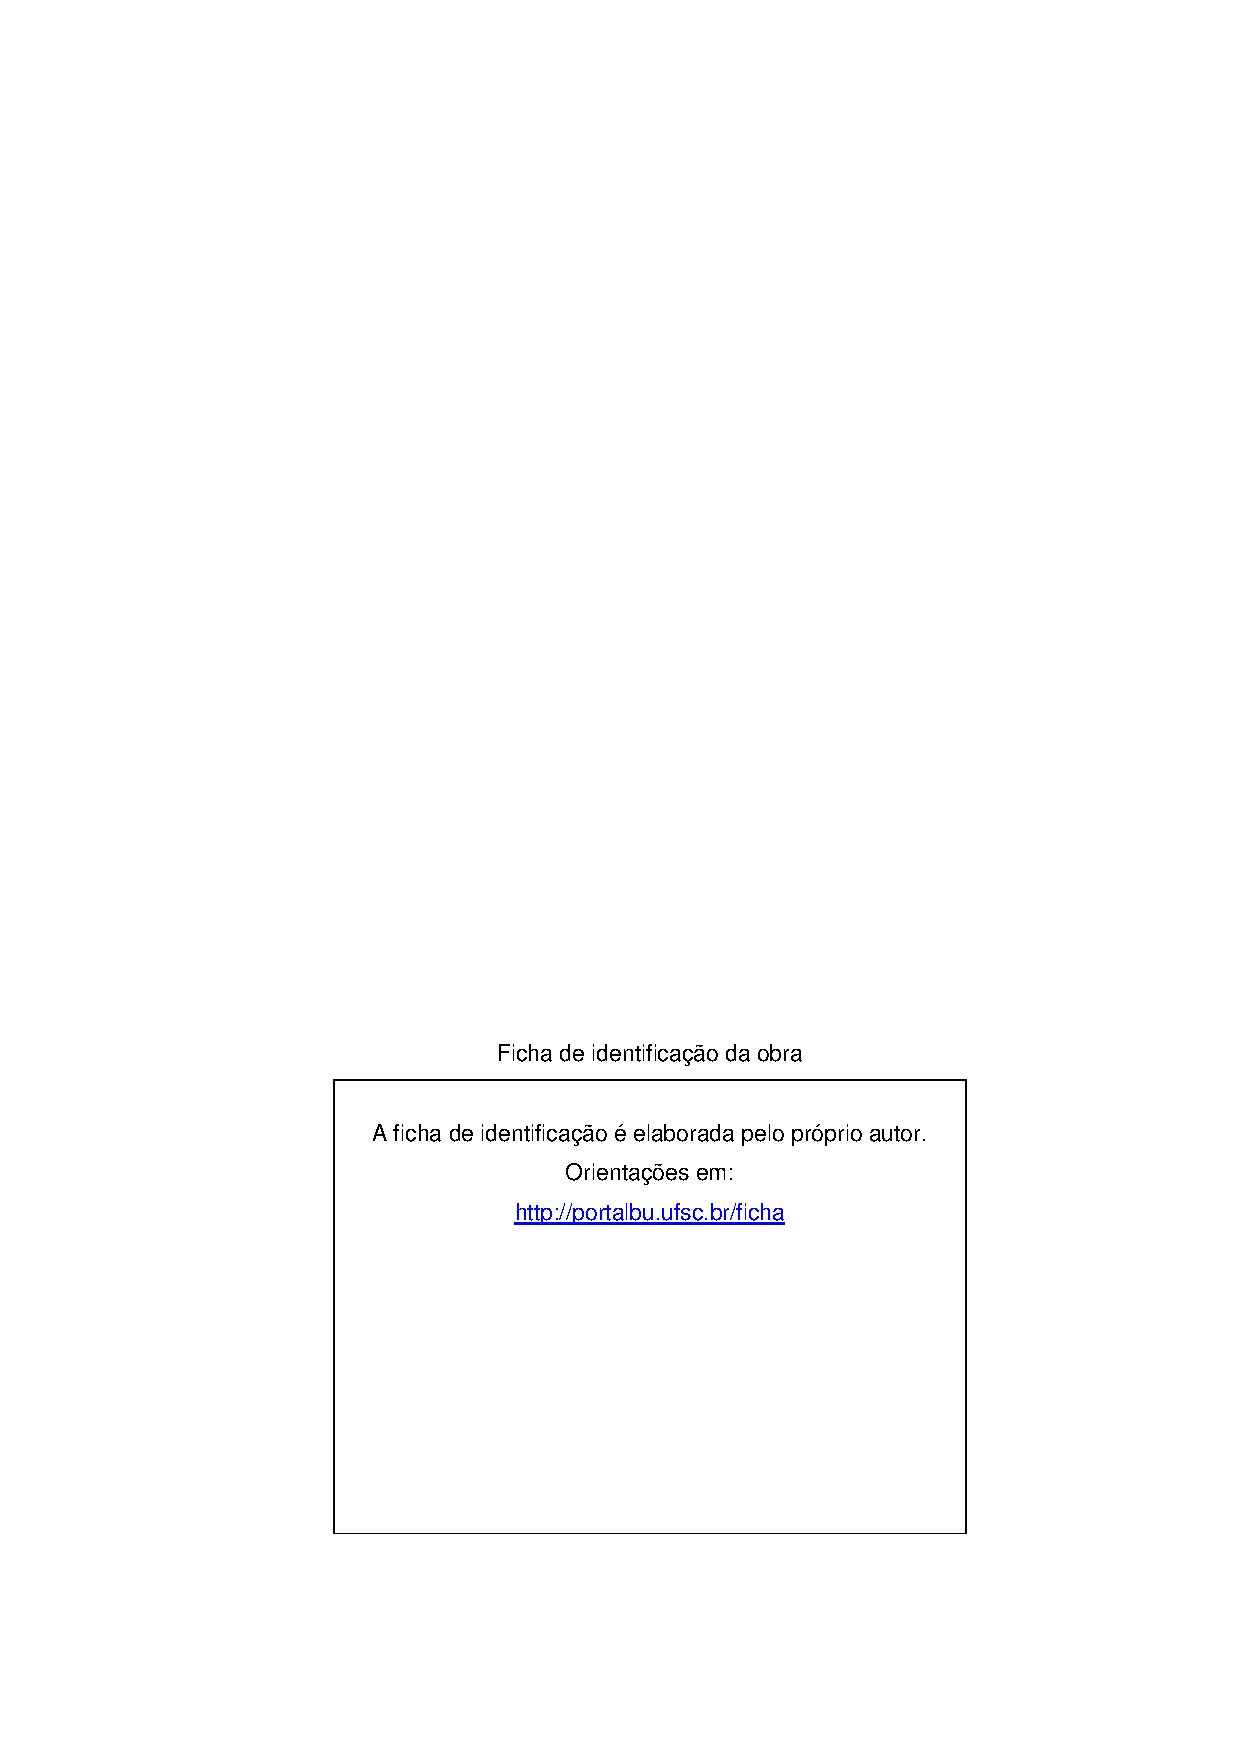
\includepdf{Ficha_Catalografica.pdf}
\end{fichacatalografica}
% ---

% ---
% Inserir folha de aprovação
% ---
\begin{folhadeaprovacao}
	\OnehalfSpacing
	\centering
	\imprimirautor\\%
	\vspace*{10pt}		
	\textbf{\imprimirtitulo}%
	\ifnotempty{\imprimirsubtitulo}{:~\imprimirsubtitulo}\\%
	%		\vspace*{31.5pt}%3\baselineskip
	\vspace*{\baselineskip}
	%\begin{minipage}{\textwidth}
	O presente trabalho em nível de \imprimirnivel~foi avaliado e aprovado por banca examinadora composta pelos seguintes membros:\\
	%\end{minipage}%
	\vspace*{\baselineskip}
    Prof. Examinador 1, Dr.\\
  Universidade Federal de Santa Catarina - UFSC\\
  \vspace*{\baselineskip}
    Prof. Examinador 2, Dr.\\
  Fédération Internationale des Géomètres - FIG\\
  \vspace*{\baselineskip}
    
	\vspace*{2\baselineskip}
	\begin{minipage}{\textwidth}
		Certificamos que esta é a \textbf{versão original e final} do trabalho de conclusão que foi julgado adequado para obtenção do título de \imprimirformacao.\\
	\end{minipage}
	%    \vspace{-0.7cm}
	\vspace*{\fill}
	\assinatura{\OnehalfSpacing Beltrano da Silva \\ Coordenação do Programa de Pós-Graduação}
	\vspace*{\fill}
	\assinatura{\OnehalfSpacing\imprimirorientador \\ \imprimirorientadorRotulo}
	%	\ifnotempty{\imprimircoorientador}{
	%	\assinatura{\imprimircoorientador \\ \imprimircoorientadorRotulo \\
	%		\imprimirinstituicao~--~\imprimirinstituicaosigla}
	%	}
	% \newpage
	\vspace*{\fill}
	\imprimirlocal, \imprimirano.
\end{folhadeaprovacao}
% ---

% ---
% Dedicatória
% ---
\begin{dedicatoria}
	\vspace*{\fill}
	\noindent
	\begin{adjustwidth*}{}{5.5cm} 
		\raggedleft       
		Este trabalho é dedicado aos meus colegas de classe e aos meus queridos pais.
	\end{adjustwidth*}
\end{dedicatoria}
% ---

% ---
% Agradecimentos
% ---
\begin{agradecimentos}
	Gostaria de agradecer sinceramente a todos os que colaboraram à execução\\
 deste trabalho.\\
 Aos colegas da UFSC.\\
 Aos professores do PPGTG.\\
 Em especial ao meu orientador, pela paciência.\\
 E a minha querida esposa pela compreensão.
\end{agradecimentos}
% ---

% ---
% Epígrafe
% ---
\begin{epigrafe}
	\vspace*{\fill}
	\begin{flushright}
		\textit{``Eppur si muove!''\\
(Galileu Galilei, 1633)}
	\end{flushright}
\end{epigrafe}
% ---

% ---
% RESUMOS
% ---

% resumo em português
\setlength{\absparsep}{18pt} % ajusta o espaçamento dos parágrafos do resumo
\begin{resumo}
	\SingleSpacing
  No resumo são ressaltados o objetivo da pesquisa, o método utilizado, as discussões e os resultados com destaque apenas para os pontos principais. O resumo deve ser significativo, composto de uma sequência de frases concisas, afirmativas, e não de uma enumeração de tópicos. Não deve conter citações. Deve usar o verbo na voz ativa e na terceira pessoa do singular. O texto do resumo deve ser digitado, em um único bloco, sem espaço de parágrafo. O espaçamento entre linhas é simples e o tamanho da fonte é 12. Abaixo do resumo, informar as palavras-chave (palavras ou expressões significativas retiradas do texto) ou, termos retirados de thesaurus da área. Deve conter de 150 a 500 palavras. O resumo é elaborado de acordo com a NBR 6028. 
  
  \textbf{Palavras-chave}: 
    Palavra-chave 1.
    Palavra-chave 2.
  \end{resumo}
% resumo em inglês
\begin{resumo}[Abstract]
	\SingleSpacing
	\begin{otherlanguage*}{english}
		Resumo traduzido para outros idiomas, neste caso, inglês. Segue o formato do resumo feito na língua vernácula. As palavras-chave traduzidas, versão em língua estrangeira, são colocadas abaixo do texto precedidas pela expressão ``Keywords'', separadas por ponto.
		
		\textbf{Keywords}:
	      Keyword 1.
        Keyword 2.
    	\end{otherlanguage*}
\end{resumo}
%% resumo em francês 
%\begin{resumo}[Résumé]
% \begin{otherlanguage*}{french}
%    Il s'agit d'un résumé en français.
% 
%   \textbf{Mots-clés}: latex. abntex. publication de textes.
% \end{otherlanguage*}
%\end{resumo}
%
%% resumo em espanhol
%\begin{resumo}[Resumen]
% \begin{otherlanguage*}{spanish}
%   Este es el resumen en español.
%  
%   \textbf{Palabras clave}: latex. abntex. publicación de textos.
% \end{otherlanguage*}
%\end{resumo}
%% ---

{%hidelinks
	\hypersetup{hidelinks}
	% ---
	% inserir lista de ilustrações
	% ---
	\pdfbookmark[0]{\listfigurename}{lof}
	\listoffigures*
	\cleardoublepage
	% ---
	
	% ---
	% inserir lista de quadros
	% ---
	\pdfbookmark[0]{\listofquadrosname}{loq}
	\listofquadros*
	\cleardoublepage
	% ---
	
	% ---
	% inserir lista de tabelas
	% ---
	\pdfbookmark[0]{\listtablename}{lot}
	\listoftables*
	\cleardoublepage
	% ---
	
	% ---
	% inserir lista de abreviaturas e siglas (devem ser declarados no preambulo)
	% ---
	\imprimirlistadesiglas
	% ---
	
	% ---
	% inserir lista de símbolos (devem ser declarados no preambulo)
	% ---
	\imprimirlistadesimbolos
	% ---
	
	% ---
	% inserir o sumario
	% ---
	\pdfbookmark[0]{\contentsname}{toc}
	\tableofcontents*
	\cleardoublepage
	
}%hidelinks
% ---

% ---

% ----------------------------------------------------------
% ELEMENTOS TEXTUAIS
% ----------------------------------------------------------
\textual

\hypertarget{intro}{%
\chapter{Introdução}\label{intro}}

Desenvolver

\hypertarget{objetivos}{%
\section{Objetivos}\label{objetivos}}

Nas seções abaixo estão descritos o objetivo geral e os objetivos
específicos.

\hypertarget{objetivo-geral}{%
\subsection{Objetivo Geral}\label{objetivo-geral}}

Descrição\ldots{}\gls{Bacen}

\hypertarget{objetivos-especuxedficos}{%
\subsection{Objetivos Específicos}\label{objetivos-especuxedficos}}

Descrição\ldots{}

\hypertarget{desenvolvimento}{%
\chapter{Desenvolvimento}\label{desenvolvimento}}

Deve-se inserir texto entre as seções.

\hypertarget{exposiuxe7uxe3o-do-tema-ou-matuxe9ria}{%
\section{Exposição do tema ou matéria\}}\label{exposiuxe7uxe3o-do-tema-ou-matuxe9ria}}

É a parte principal e mais extensa do trabalho. Deve apresentar a fundamentação
teórica, a metodologia, os resultados e a discussão. Divide-se em seções e
subseções conforme a NBR 6024 \autocite*{NBR6024:2012} - ver figura \ref{fig:imagem}.

Quanto à sua estrutura e projeto gráfico, segue as recomendações da \gls{ABNT}
para preparação de trabalhos acadêmicos, a NBR 14724 \autocite*{NBR14724:2011}.
\begin{figure}[H]

{\centering 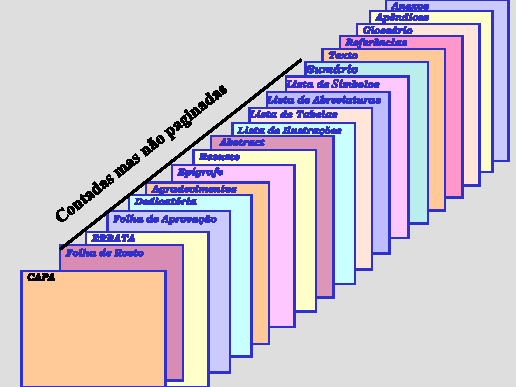
\includegraphics[width=0.7\linewidth]{images/imagem} 

}

\caption{Elementos do trabalho acadêmico.}\label{fig:imagem}
\end{figure}
\bcenter

Fonte: Universidade Federal do Paraná (1996).
\ecenter

\hypertarget{formatauxe7uxe3o-do-texto}{%
\subsection{Formatação do texto}\label{formatauxe7uxe3o-do-texto}}

No que diz respeito à estrutura do trabalho, recomenda-se que:
\begin{enumerate}
\def\labelenumi{\alph{enumi}.}
\tightlist
\item
  o texto deve ser justificado, digitado em cor preta, podendo utilizar outras
  cores somente para as ilustrações;
\item
  utilizar papel branco ou reciclado para impressão;
\item
  os elementos pré-textuais devem iniciar no anverso da folha, com exceção da
  ficha catalográfica ou ficha de identificação da obra;
\item
  os elementos textuais e pós-textuais devem ser digitados no anverso e verso
  das folhas, quando o trabalho for impresso. As seções primárias devem começar
  sempre em páginas ímpares, quando o trabalho for impresso. Deixar um espaço
  entre o título da seção/subseção e o texto e entre o texto e o título da subseção.
\end{enumerate}
No Quadro \ref{qua:Quadro-1} estão as especificações para a formatação do texto.
\begin{quadro}[htb]
    \centering
    \caption{\label{qua:Quadro-1}Formatação do texto.}  
    \begin{tabular}{|l|p{11cm}|}
        \hline
        \textbf{Formato do papel} & A4.\\ \hline
        \textbf{Impressão}        & A norma recomenda que caso seja necessário imprimir, deve-se utilizar a frente e o verso da página.\\ \hline
        \textbf{Margens}          & Superior: 3, Inferior: 2, Interna: 3 e Externa: 2. Usar margens espelhadas quando o  trabalho for impresso.\\ \hline
        \textbf{Paginação}        & As páginas dos elementos pré-textuais devem ser contadas, mas não numeradas. Para trabalhos digitados somente no anverso, a numeração das páginas deve constar no canto superior direito da página, a 2 cm da borda, figurando a partir da primeira folha da  parte textual. Para trabalhos digitados no anverso e no verso, a numeração deve constar no canto superior direito, no anverso, e no canto superior esquerdo no verso.\\ \hline
        \textbf{Espaçamento}      & O texto deve ser redigido com espaçamento entre linhas 1,5, excetuando-se as citações de mais de três linhas, notas de rodapé, referências, legendas das ilustrações e das tabelas, natureza (tipo do trabalho, objetivo, nome da instituição a que é submetido e área de concentração), que devem ser digitados em espaço simples, com fonte menor. As referências devem ser separadas entre si por um espaço simples em branco.\\ \hline
        \textbf{Paginação}        & A contagem inicia na folha de rosto, mas se insere o número da página na introdução até o final do trabalho.\\ \hline
        \textbf{Fontes sugeridas} & Arial ou Times New Roman.\\ \hline
        \textbf{Tamanho da fonte} & \textbf{Fonte tamanho 12 para o texto}, incluindo os títulos das seções e subseções. As citações com mais de três linhas, notas de rodapé, paginação, dados internacionais de catalogação, legendas e fontes das ilustrações e das tabelas devem ser de tamanho menor. Adotamos, neste \textit{template} \textbf{fonte tamanho 10}.\\ \hline
        \textbf{Nota de rodapé}   & Devem ser digitadas dentro da margem, ficando separadas por um espaço simples por entre as linhas e por filete de 5 cm a partir da margem esquerda. A partir da segunda linha, devem ser alinhadas embaixo da primeira letra da primeira palavra da primeira linha.\\ \hline
    \end{tabular}
    \fonte{\textcite{NBR14724:2011}.}
\end{quadro}
\hypertarget{as-ilustrauxe7uxf5es}{%
\subsection{As ilustrações}\label{as-ilustrauxe7uxf5es}}

Independentemente do tipo de ilustração (quadro, desenho, figura, fotografia,
mapa, entre outros), a sua identificação aparece na parte superior, precedida da
palavra designativa.
\begin{quote}
Após a ilustração, na parte inferior, indicar a fonte consultada (elemento
obrigatório, mesmo que seja produção do próprio autor), legenda, notas e outras
informações necessárias à sua compreensão (se houver). A ilustração deve ser
citada no texto e inserida o mais próximo possível do texto a que se refere.

--- \autocite[11]{NBR14724:2011}.
\end{quote}
\hypertarget{equauxe7uxf5es-e-fuxf3rmulas}{%
\subsubsection{Equações e fórmulas}\label{equauxe7uxf5es-e-fuxf3rmulas}}

As equações e fórmulas devem ser destacadas no texto para facilitar a leitura.
Para numerá-las, usar algarismos arábicos entre parênteses e alinhados à direita.
Pode-se adotar uma entrelinha maior do que a usada no texto \autocite{NBR14724:2011}.

Exemplos, equação \eqref{eq:eq-1} e equação \eqref{eq:eq-2}.
\begin{equation}
  \gls{C} = 2 \gls{pi} \gls{r}
  \label{eq:eq-1}
\end{equation}
\begin{equation}
  \gls{A} = \gls{pi} \gls{r}^2
  \label{eq:eq-2}
\end{equation}
\hypertarget{exemplo-tabela}{%
\paragraph{Exemplo tabela}\label{exemplo-tabela}}

De acordo com \textcite{ibge1993}, tabela é uma forma não discursiva de apresentar
informações em que os números representam a informação central.
Ver tabela \ref{tab:tab-1}.
\begin{table}[htb]
    \ABNTEXfontereduzida
    \caption{\label{tab:tab-1}Médias concentrações urbanas 2010-2011.}
    \begin{tabular}{@{}p{3.0cm}p{1.5cm}p{2cm}p{2.5cm}p{2.5cm}p{2.5cm}@{}}
        \toprule
        \textbf{Média concentração urbana} & \multicolumn{2}{l}{\textbf{População}} & \textbf{Produto Interno Bruto – PIB (bilhões R\$)} & \textbf{Número de empresas} & \textbf{Número de unidades locais} \\ \midrule
        \textbf{Nome}                      & \textbf{Total}   & \textbf{No Brasil}  &                                                   &                             & \\
        Ji-Paraná (RO)                     & 116 610          & 116 610             & 1,686                                             & 2 734                       & 3 082 \\
        Parintins (AM)                     & 102 033          & 102 033             & 0,675                                             & 634                         & 683 \\
        Boa Vista (RR)                     & 298 215          & 298 215             & 4,823                                             & 4 852                       & 5 187 \\
        Bragança (PA)                      & 113 227          & 113 227             & 0,452                                             & 654                         & 686 \\ \bottomrule
    \end{tabular}
\end{table}
\bcenter

Fonte: \textcite{ibge2016}
\ecenter

As tabelas podem ser escritas em código latex, como acima.

Porém, é recomendável utilizar o \proglang{R} para produzí-las, através dos pacotes
\pkg{knitr} e \pkg{kableExtra}. Para isto é necessário inserir os dados no
\proglang{R}, como abaixo, ou através da leitura de um arquivo de dados.

O código de geração da tabela \ref{tab:media-concentracao-urbana} pode ser
visto no Apêndice \ref{appendix-a}.
\begin{table}

\caption{\label{tab:media-concentracao-urbana}Médias concentrações urbanas 2010-2011.}
\centering
\begin{tabular}[t]{lrr>{\raggedleft\arraybackslash}p{1.5cm}>{\raggedleft\arraybackslash}p{1.5cm}>{\raggedleft\arraybackslash}p{1.5cm}}
\toprule
\multicolumn{1}{c}{\textbf{Média Concentração Urbana}} & \multicolumn{2}{c}{\textbf{População}} \\
\cmidrule(l{3pt}r{3pt}){1-1} \cmidrule(l{3pt}r{3pt}){2-3}
\textbf{Nome} & \textbf{Total} & \textbf{No Brasil} & \textbf{Produto Interno Bruto - PIB} & \textbf{Número de Empresas} & \textbf{Número de unidades locais}\\
\midrule
\cellcolor{gray!6}{Ji-Paraná (RO)} & \cellcolor{gray!6}{116 610} & \cellcolor{gray!6}{116 610} & \cellcolor{gray!6}{1,686} & \cellcolor{gray!6}{2 734} & \cellcolor{gray!6}{3 082}\\
Parintins (AM) & 102 033 & 102 033 & 0,675 & 634 & 683\\
\cellcolor{gray!6}{Boa Vista (RR)} & \cellcolor{gray!6}{298 215} & \cellcolor{gray!6}{298 215} & \cellcolor{gray!6}{4,823} & \cellcolor{gray!6}{4 852} & \cellcolor{gray!6}{5 187}\\
Bragança (PA) & 113 227 & 113 227 & 0,452 & 654 & 686\\
\bottomrule
\multicolumn{6}{l}{\rule{0pt}{1em}\textit{Notas:}}\\
\multicolumn{6}{l}{\rule{0pt}{1em}PIB em bilhões de reais.}\\
\multicolumn{6}{l}{\rule{0pt}{1em}Fonte: IBGE (2016)}\\
\end{tabular}
\end{table}
Outra maneira, ainda, para tabelas mais simples, como a tabela \ref{tab:inher},
é inserí-las no formato Pandoc (ver a
\href{https://pandoc.org/MANUAL.html\#tables}{documentação do pandoc} para mais detalhes).
\begin{longtable}[]{@{}
  >{\centering\arraybackslash}p{(\columnwidth - 4\tabcolsep) * \real{0.3133}}
  >{\centering\arraybackslash}p{(\columnwidth - 4\tabcolsep) * \real{0.5060}}
  >{\centering\arraybackslash}p{(\columnwidth - 4\tabcolsep) * \real{0.1807}}@{}}
\caption{\label{tab:inher} Correlation of Inheritance Factors for Parents and Child}\tabularnewline
\toprule
\begin{minipage}[b]{\linewidth}\centering
Factors
\end{minipage} & \begin{minipage}[b]{\linewidth}\centering
Correlation between Parents \& Child
\end{minipage} & \begin{minipage}[b]{\linewidth}\centering
Inherited
\end{minipage} \\
\midrule
\endfirsthead
\toprule
\begin{minipage}[b]{\linewidth}\centering
Factors
\end{minipage} & \begin{minipage}[b]{\linewidth}\centering
Correlation between Parents \& Child
\end{minipage} & \begin{minipage}[b]{\linewidth}\centering
Inherited
\end{minipage} \\
\midrule
\endhead
Education & -0.49 & Yes \\
Socio-Economic Status & 0.28 & Slight \\
Income & 0.08 & No \\
Family Size & 0.18 & Slight \\
Occupational Prestige & 0.21 & Slight \\
\bottomrule
\end{longtable}
\bcenter

Fonte: do Autor.
\ecenter

\hypertarget{plots}{%
\chapter{Plots}\label{plots}}

Este \emph{template} contém algumas seções criadas na tentativa de facilitar seu uso.
No entanto, não há um limite máximo ou mínimo de seção a ser utilizado no
trabalho. Cabe a cada autor definir a quantidade que melhor atenda à sua
necessidade.

Para criar figuras com o \proglang{R}, pode-se seguir o padrão do código
abaixo, utilizado para produzir as imagens da figura \ref{fig:anscombe}:
\begin{Shaded}
\begin{Highlighting}[]
\FunctionTok{data}\NormalTok{(anscombe)}
\FunctionTok{plot}\NormalTok{(y1}\SpecialCharTok{\textasciitilde{}}\NormalTok{x1, }\AttributeTok{data =}\NormalTok{ anscombe)}
\FunctionTok{abline}\NormalTok{(}\FunctionTok{lm}\NormalTok{(y1}\SpecialCharTok{\textasciitilde{}}\NormalTok{x1, }\AttributeTok{data =}\NormalTok{ anscombe))}
\FunctionTok{plot}\NormalTok{(y2}\SpecialCharTok{\textasciitilde{}}\NormalTok{x2, }\AttributeTok{data =}\NormalTok{ anscombe)}
\FunctionTok{abline}\NormalTok{(}\FunctionTok{lm}\NormalTok{(y2}\SpecialCharTok{\textasciitilde{}}\NormalTok{x2, }\AttributeTok{data =}\NormalTok{ anscombe))}
\FunctionTok{plot}\NormalTok{(y3}\SpecialCharTok{\textasciitilde{}}\NormalTok{x3, }\AttributeTok{data =}\NormalTok{ anscombe)}
\FunctionTok{abline}\NormalTok{(}\FunctionTok{lm}\NormalTok{(y3}\SpecialCharTok{\textasciitilde{}}\NormalTok{x3, }\AttributeTok{data =}\NormalTok{ anscombe))}
\FunctionTok{plot}\NormalTok{(y4}\SpecialCharTok{\textasciitilde{}}\NormalTok{x4, }\AttributeTok{data =}\NormalTok{ anscombe)}
\FunctionTok{abline}\NormalTok{(}\FunctionTok{lm}\NormalTok{(y4}\SpecialCharTok{\textasciitilde{}}\NormalTok{x4, }\AttributeTok{data =}\NormalTok{ anscombe))}
\end{Highlighting}
\end{Shaded}
\begin{figure}[H]

{\centering 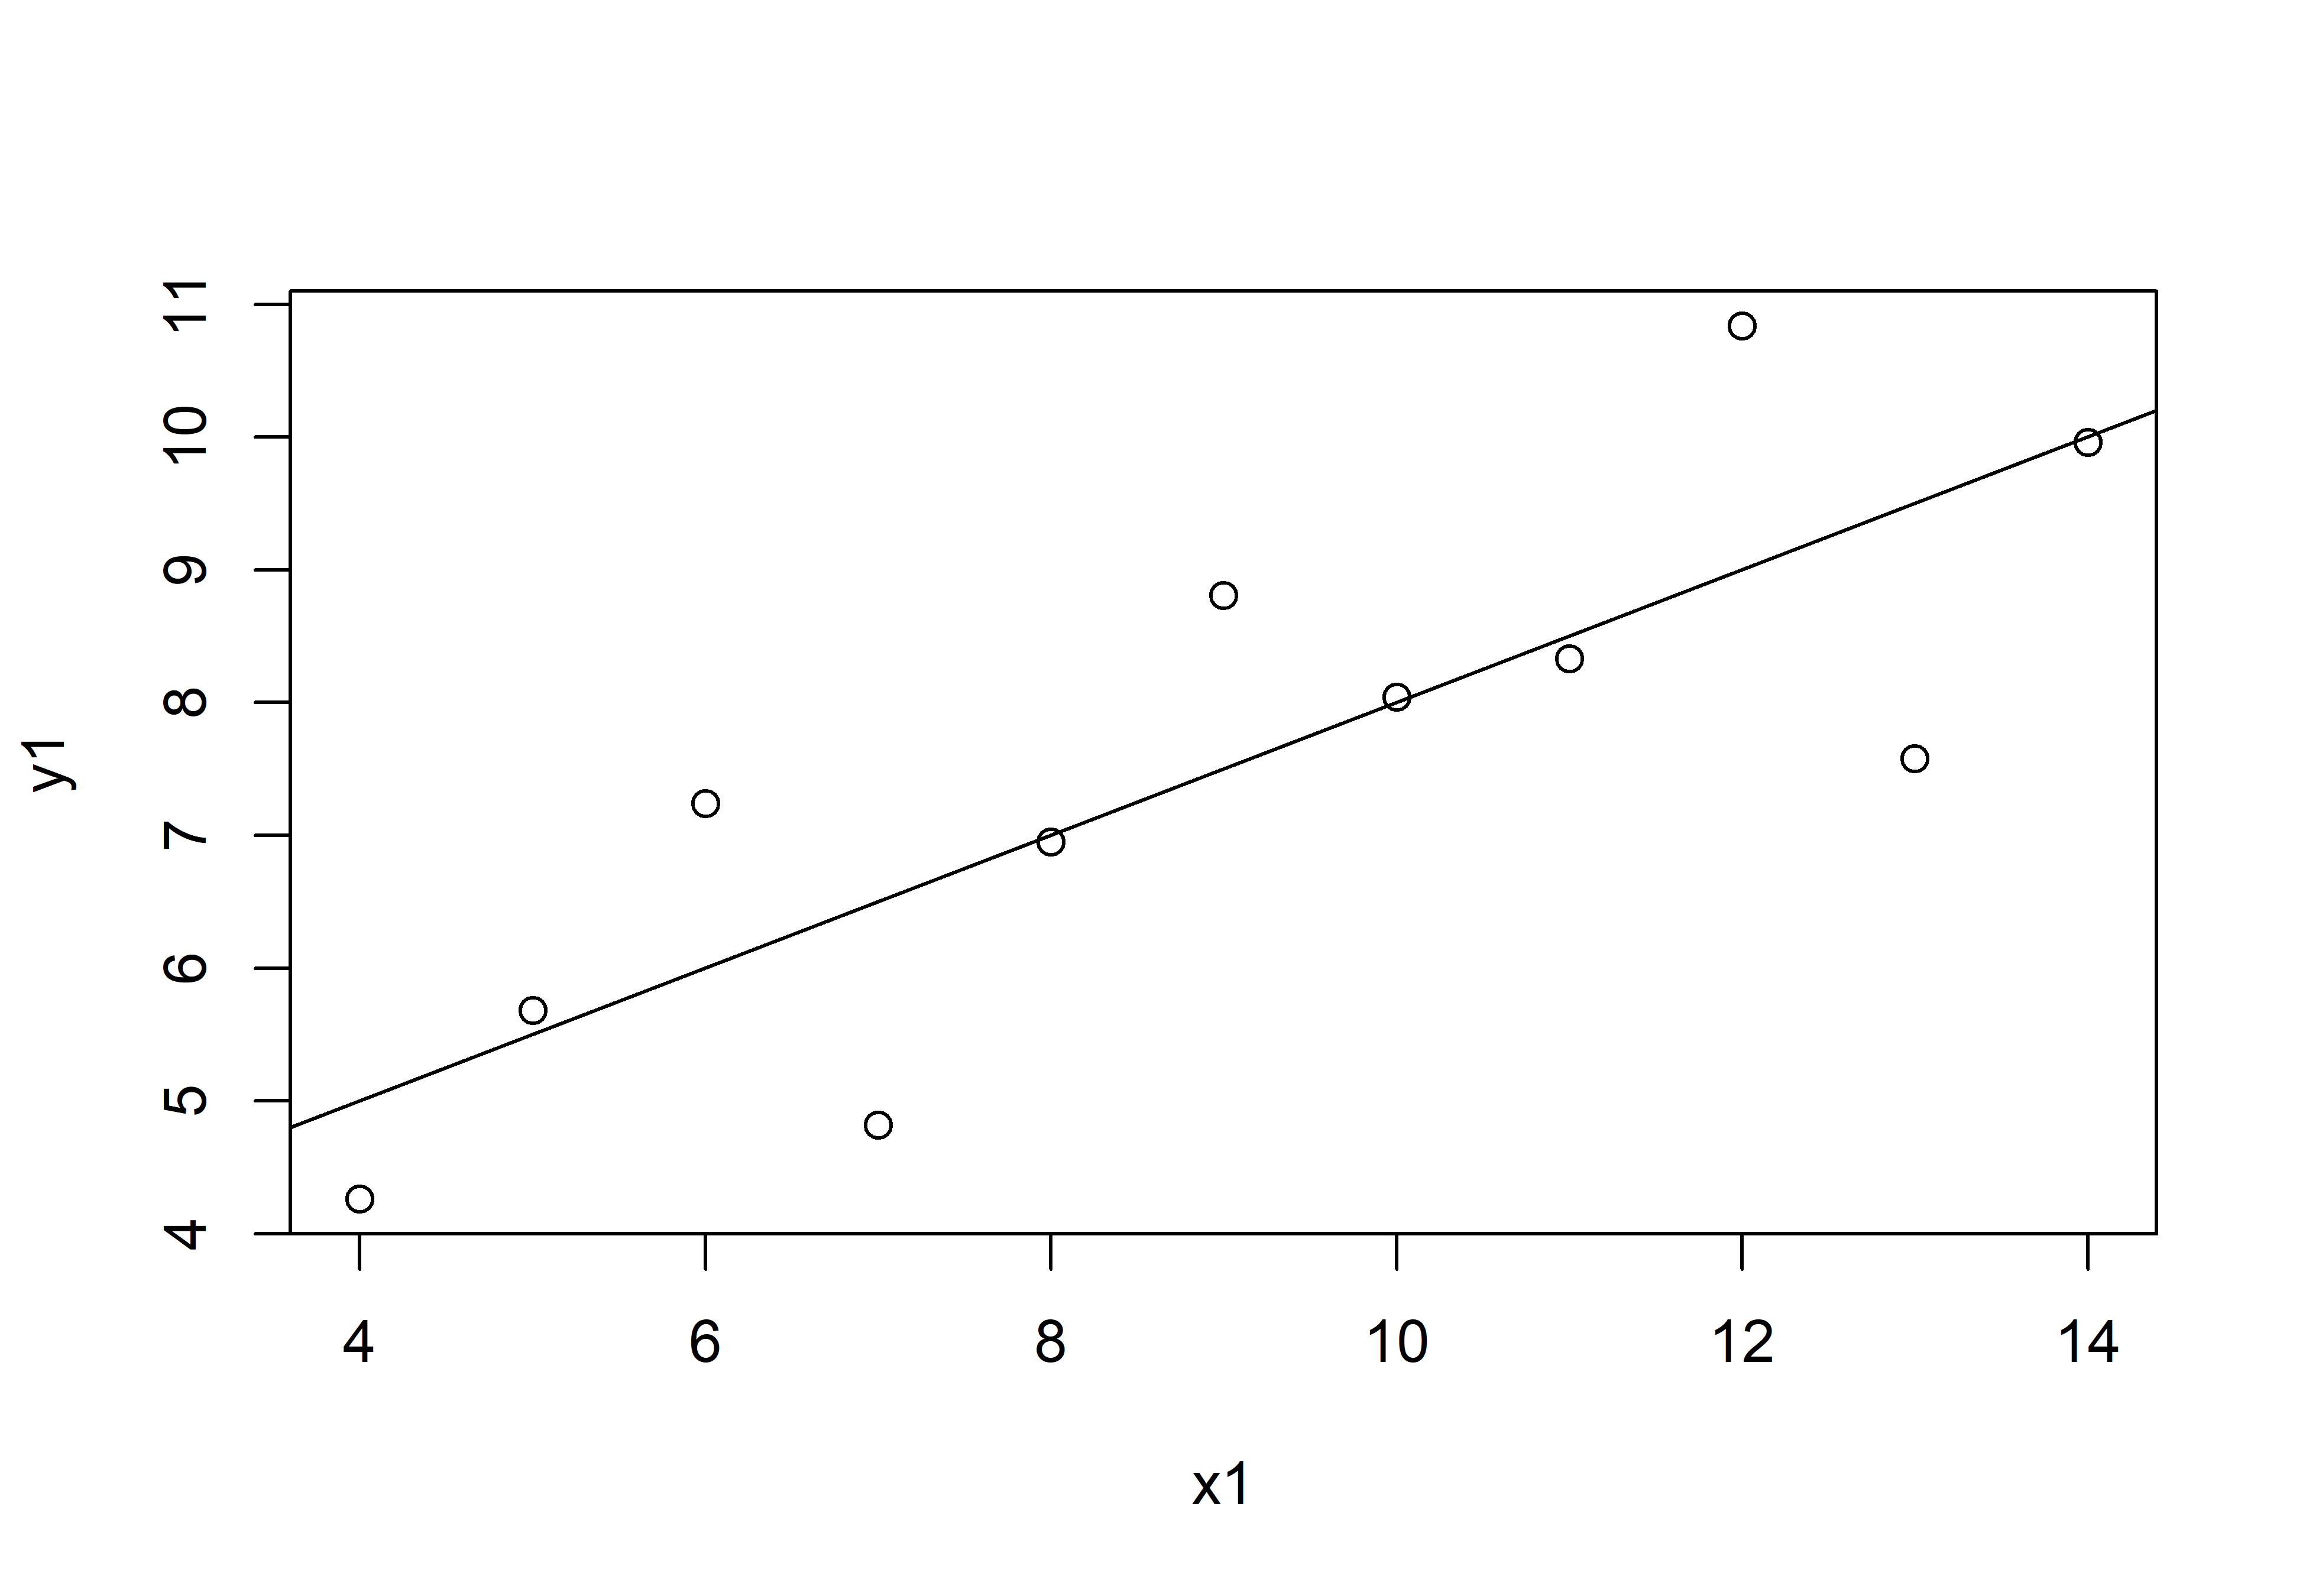
\includegraphics[width=0.49\linewidth]{images/anscombe-1} 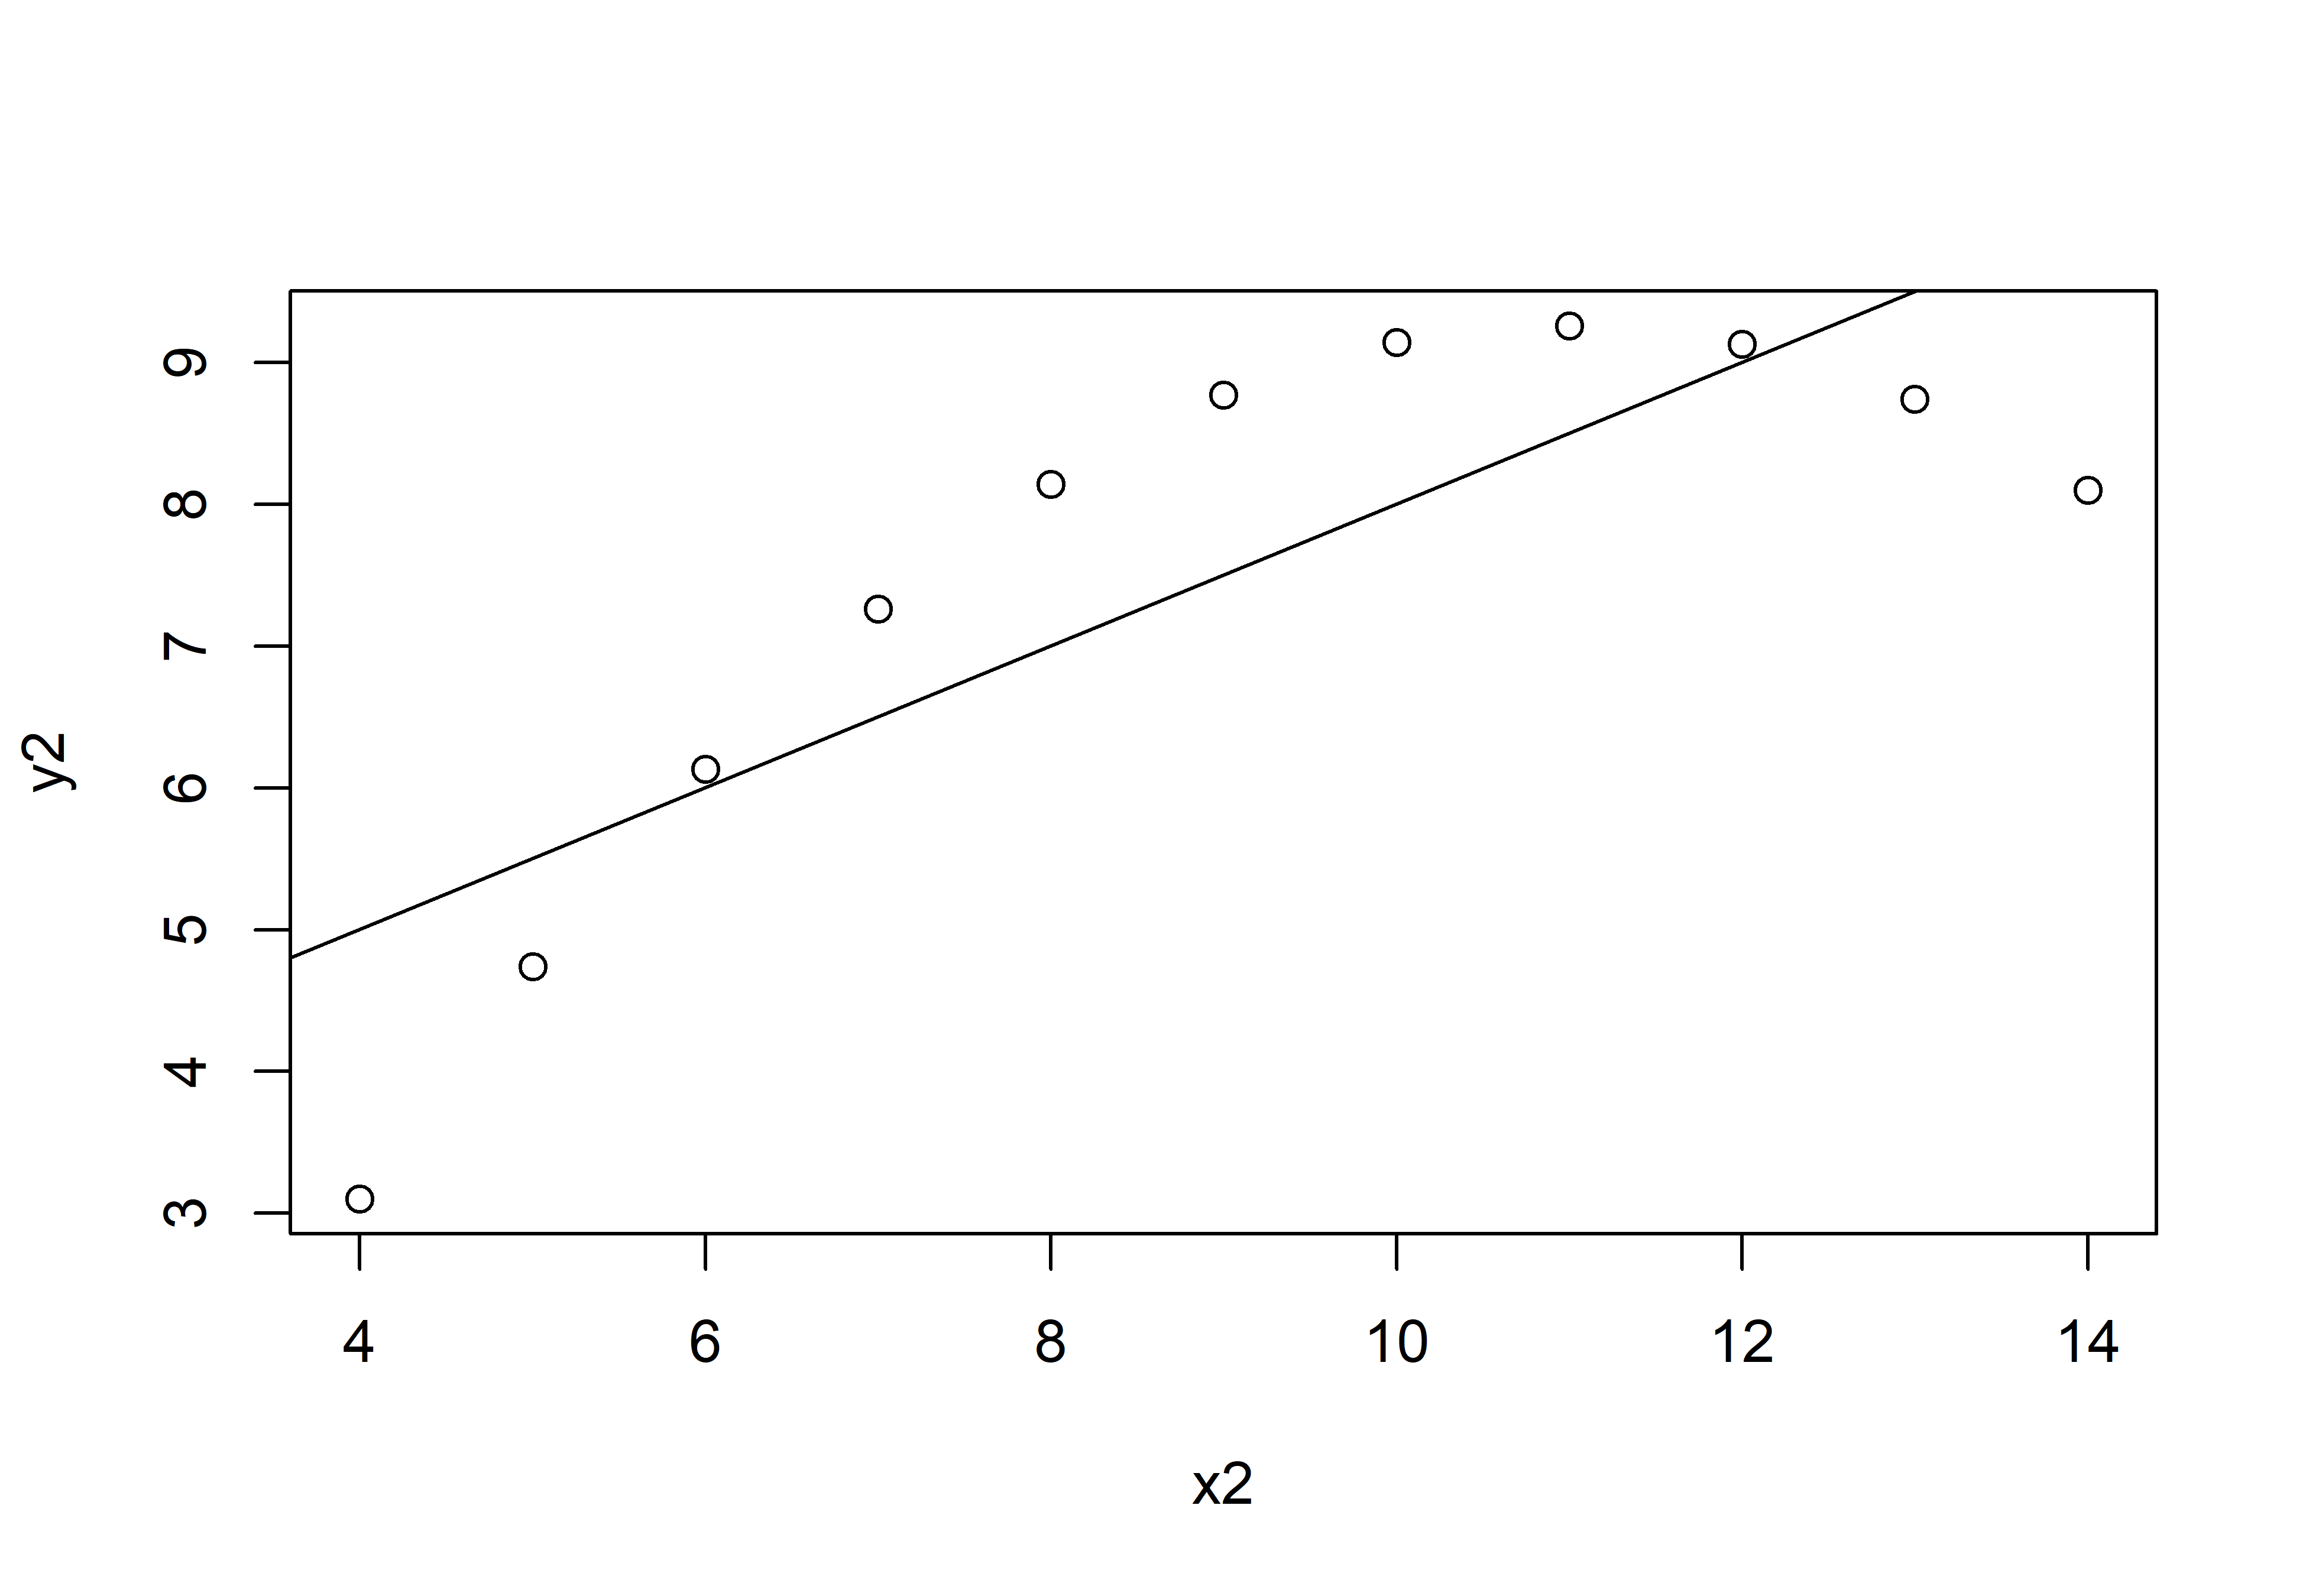
\includegraphics[width=0.49\linewidth]{images/anscombe-2} 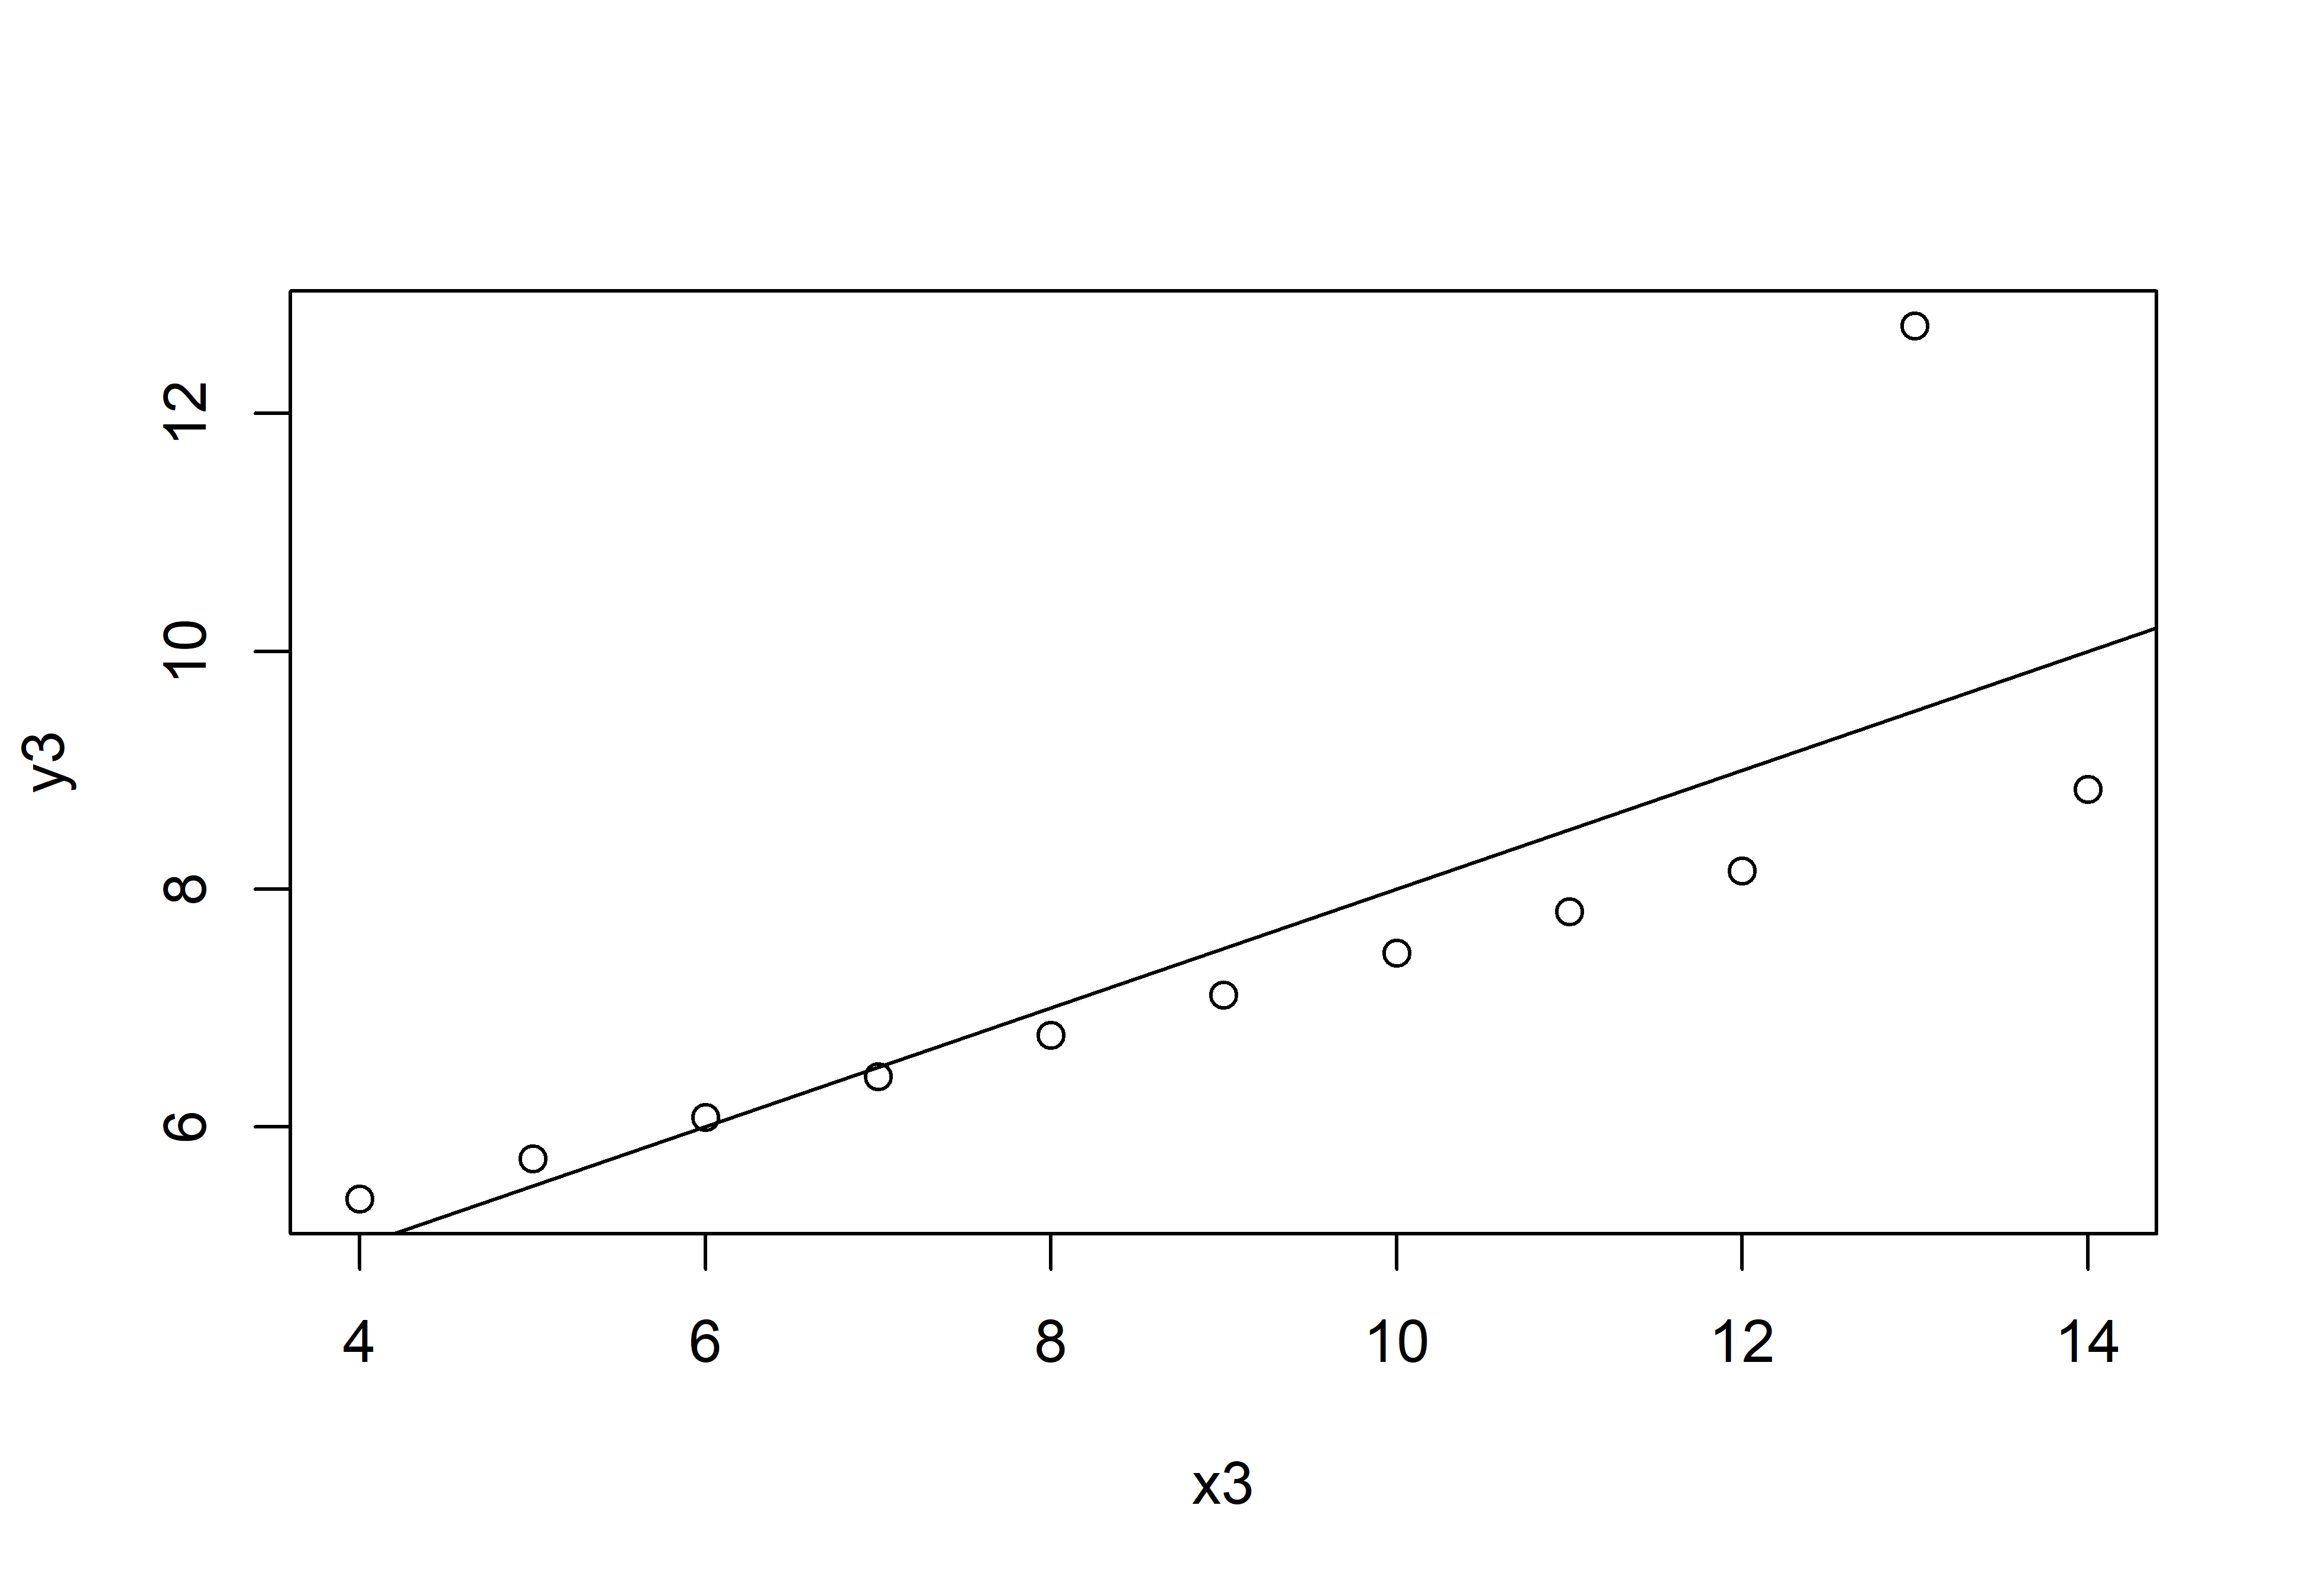
\includegraphics[width=0.49\linewidth]{images/anscombe-3} 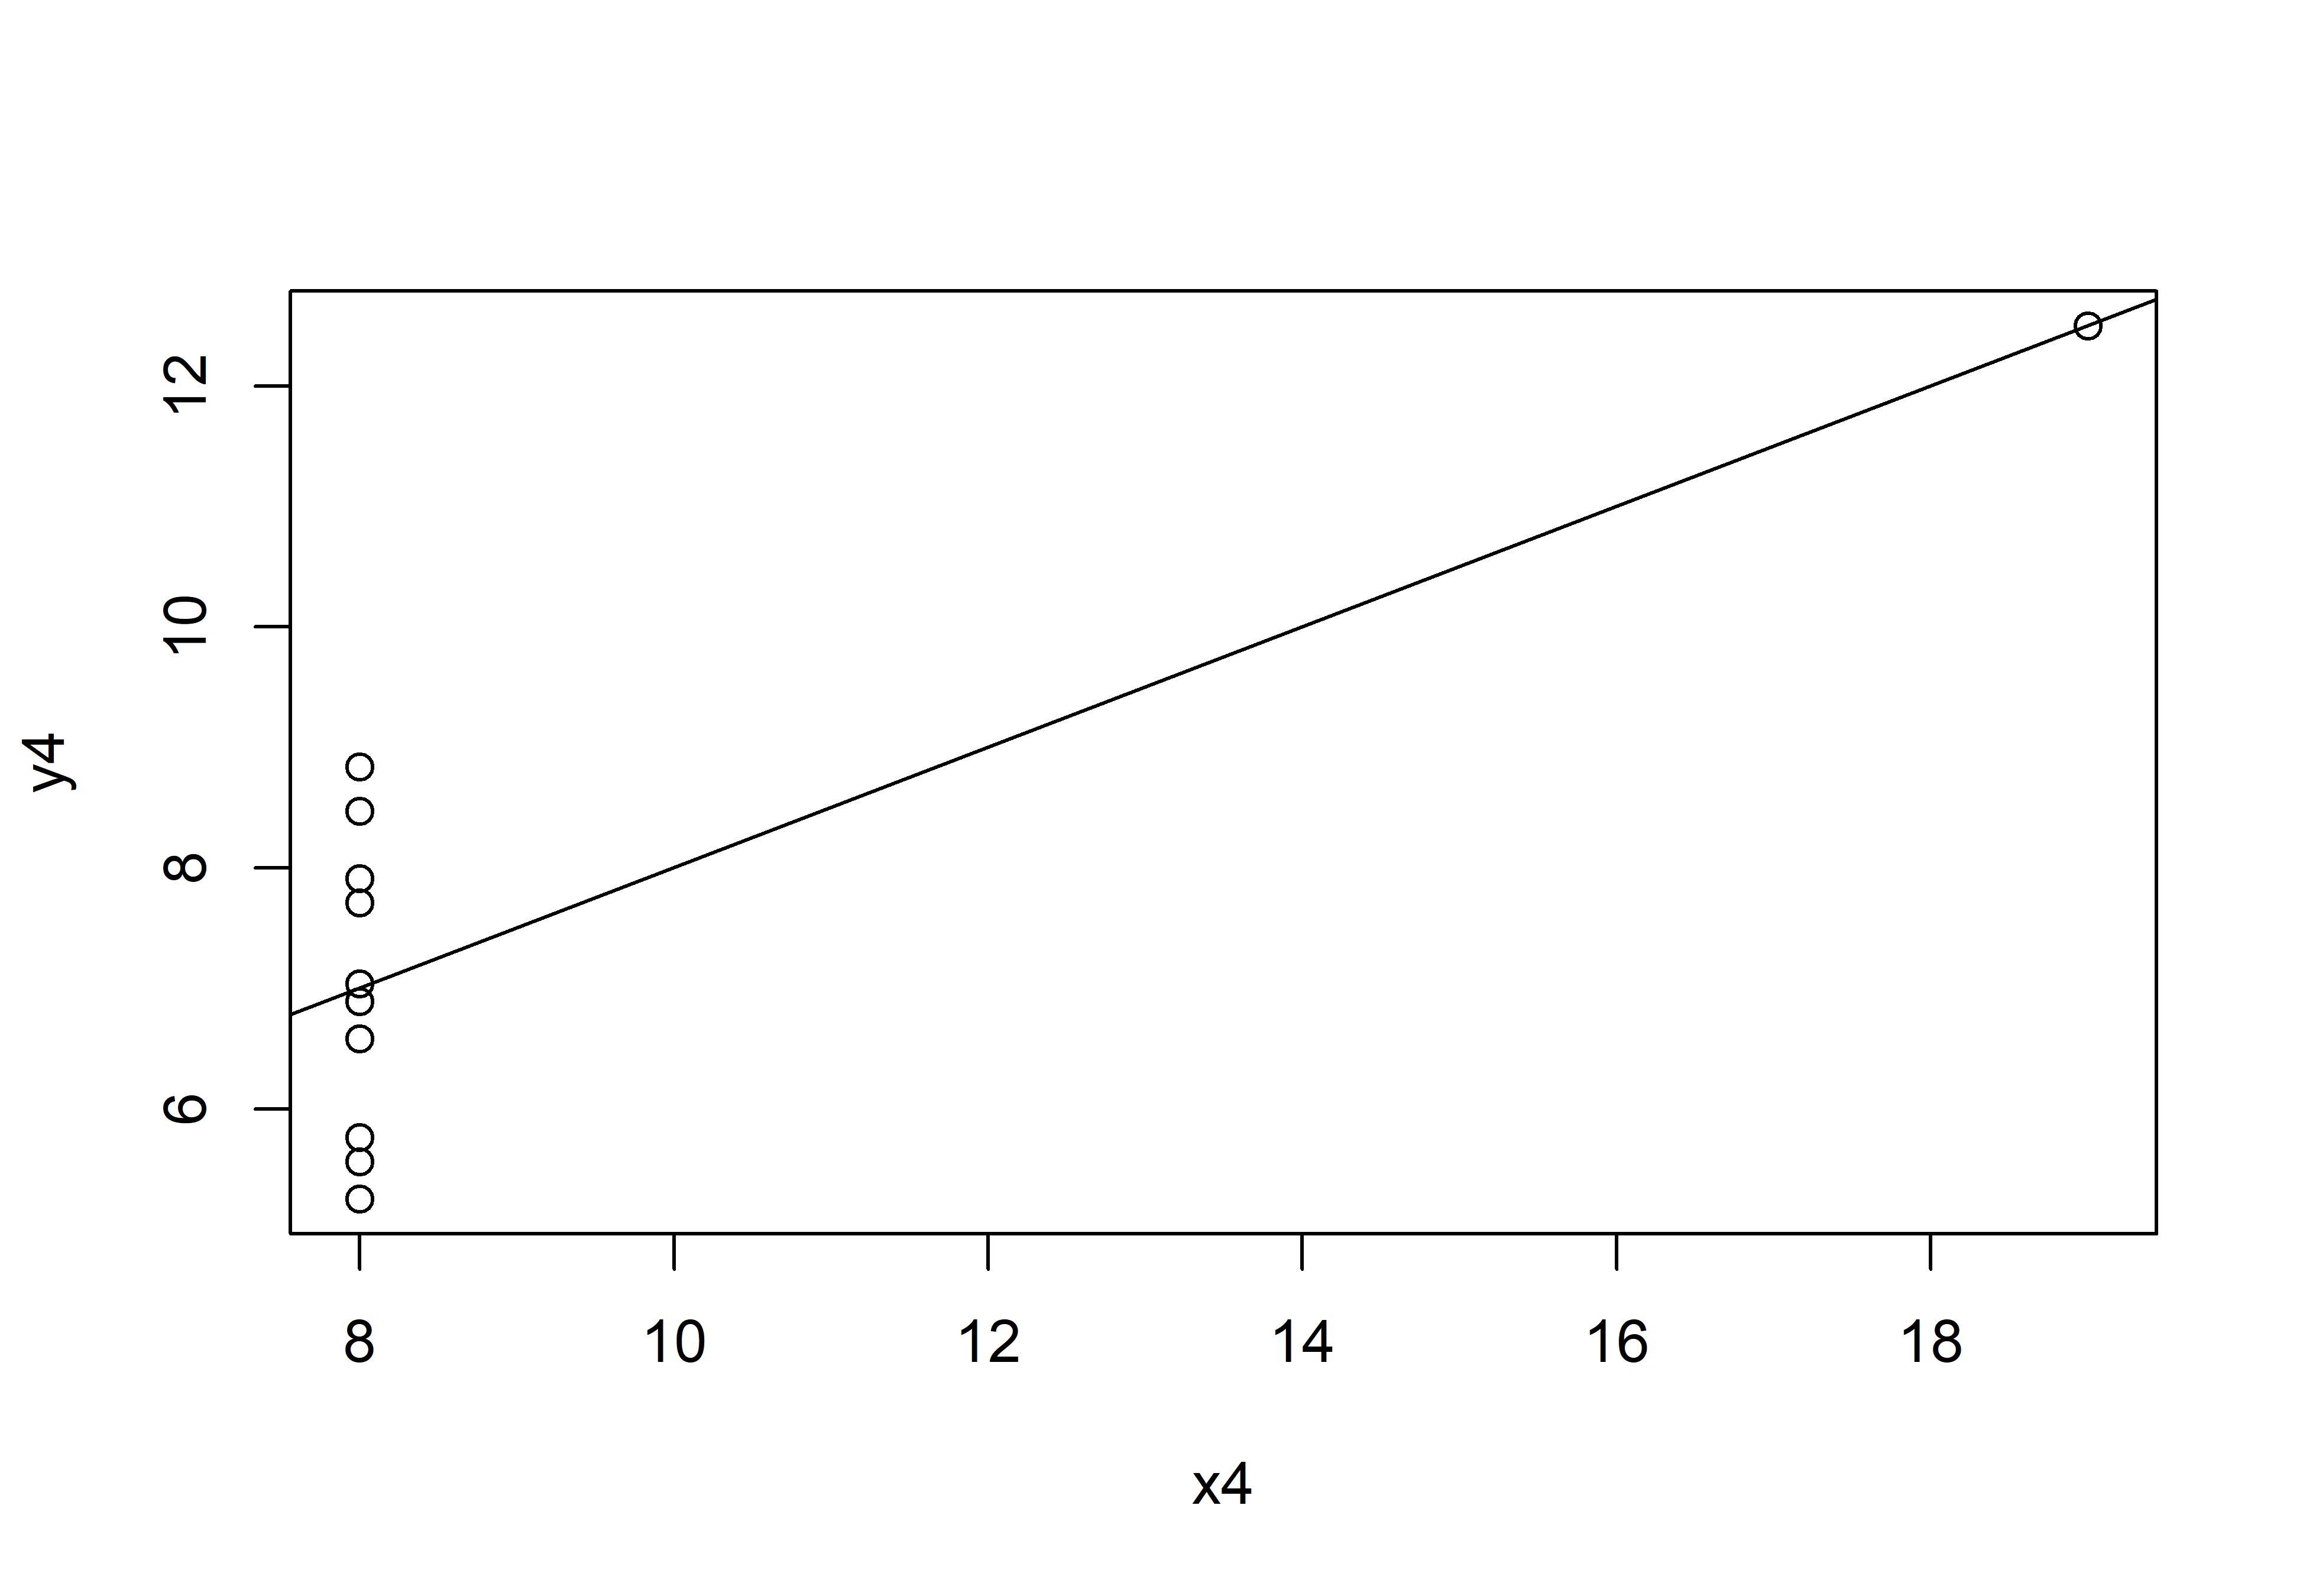
\includegraphics[width=0.49\linewidth]{images/anscombe-4} 

}

\caption{O quarteto de Anscombe.}\label{fig:anscombe}
\end{figure}
\bcenter

Fonte: do Autor.
\ecenter

Ou utilizando o pacote \pkg{ggplot2} \autocite*{R-ggplot2}, obtendo-se a figura \ref{fig:anscombe2}.
\begin{Shaded}
\begin{Highlighting}[]
\FunctionTok{library}\NormalTok{(ggplot2)}
\NormalTok{p1 }\OtherTok{\textless{}{-}} \FunctionTok{ggplot}\NormalTok{(anscombe, }\FunctionTok{aes}\NormalTok{(}\AttributeTok{x =}\NormalTok{ x1, }\AttributeTok{y =}\NormalTok{ y1)) }\SpecialCharTok{+}
  \FunctionTok{geom\_point}\NormalTok{(}\AttributeTok{color =} \StringTok{"darkorange"}\NormalTok{, }\AttributeTok{size =} \FloatTok{1.5}\NormalTok{) }\SpecialCharTok{+}
  \FunctionTok{scale\_x\_continuous}\NormalTok{(}\AttributeTok{breaks =} \FunctionTok{seq}\NormalTok{(}\DecValTok{0}\NormalTok{,}\DecValTok{20}\NormalTok{,}\DecValTok{2}\NormalTok{)) }\SpecialCharTok{+}
  \FunctionTok{scale\_y\_continuous}\NormalTok{(}\AttributeTok{breaks =} \FunctionTok{seq}\NormalTok{(}\DecValTok{0}\NormalTok{,}\DecValTok{12}\NormalTok{,}\DecValTok{2}\NormalTok{)) }\SpecialCharTok{+}
  \FunctionTok{expand\_limits}\NormalTok{(}\AttributeTok{x =} \DecValTok{0}\NormalTok{, }\AttributeTok{y =} \DecValTok{0}\NormalTok{) }\SpecialCharTok{+}
  \FunctionTok{labs}\NormalTok{(}\AttributeTok{x =} \StringTok{"x1"}\NormalTok{, }\AttributeTok{y =} \StringTok{"y1"}\NormalTok{,}
       \AttributeTok{title =} \StringTok{"Dataset 1"}\NormalTok{ ) }\SpecialCharTok{+}
  \FunctionTok{geom\_smooth}\NormalTok{(}\AttributeTok{method =} \StringTok{"lm"}\NormalTok{, }\AttributeTok{se =} \ConstantTok{FALSE}\NormalTok{)}

\NormalTok{p2 }\OtherTok{\textless{}{-}} \FunctionTok{ggplot}\NormalTok{(anscombe, }\FunctionTok{aes}\NormalTok{(}\AttributeTok{x =}\NormalTok{ x2, }\AttributeTok{y =}\NormalTok{ y2)) }\SpecialCharTok{+}
  \FunctionTok{geom\_point}\NormalTok{(}\AttributeTok{color =} \StringTok{"darkorange"}\NormalTok{, }\AttributeTok{size =} \FloatTok{1.5}\NormalTok{) }\SpecialCharTok{+}
  \FunctionTok{scale\_x\_continuous}\NormalTok{(}\AttributeTok{breaks =} \FunctionTok{seq}\NormalTok{(}\DecValTok{0}\NormalTok{,}\DecValTok{20}\NormalTok{,}\DecValTok{2}\NormalTok{)) }\SpecialCharTok{+}
  \FunctionTok{scale\_y\_continuous}\NormalTok{(}\AttributeTok{breaks =} \FunctionTok{seq}\NormalTok{(}\DecValTok{0}\NormalTok{,}\DecValTok{12}\NormalTok{,}\DecValTok{2}\NormalTok{)) }\SpecialCharTok{+}
  \FunctionTok{expand\_limits}\NormalTok{(}\AttributeTok{x =} \DecValTok{0}\NormalTok{, }\AttributeTok{y =} \DecValTok{0}\NormalTok{) }\SpecialCharTok{+}
  \FunctionTok{labs}\NormalTok{(}\AttributeTok{x =} \StringTok{"x2"}\NormalTok{, }\AttributeTok{y =} \StringTok{"y2"}\NormalTok{,}
       \AttributeTok{title =} \StringTok{"Dataset 2"}\NormalTok{ ) }\SpecialCharTok{+}
  \FunctionTok{geom\_smooth}\NormalTok{(}\AttributeTok{method =} \StringTok{"lm"}\NormalTok{, }\AttributeTok{se =} \ConstantTok{FALSE}\NormalTok{)}

\NormalTok{p3 }\OtherTok{\textless{}{-}} \FunctionTok{ggplot}\NormalTok{(anscombe, }\FunctionTok{aes}\NormalTok{(}\AttributeTok{x =}\NormalTok{ x3, }\AttributeTok{y =}\NormalTok{ y3)) }\SpecialCharTok{+}
  \FunctionTok{geom\_point}\NormalTok{(}\AttributeTok{color =} \StringTok{"darkorange"}\NormalTok{, }\AttributeTok{size =} \FloatTok{1.5}\NormalTok{) }\SpecialCharTok{+}
  \FunctionTok{scale\_x\_continuous}\NormalTok{(}\AttributeTok{breaks =} \FunctionTok{seq}\NormalTok{(}\DecValTok{0}\NormalTok{,}\DecValTok{20}\NormalTok{,}\DecValTok{2}\NormalTok{)) }\SpecialCharTok{+}
  \FunctionTok{scale\_y\_continuous}\NormalTok{(}\AttributeTok{breaks =} \FunctionTok{seq}\NormalTok{(}\DecValTok{0}\NormalTok{,}\DecValTok{12}\NormalTok{,}\DecValTok{2}\NormalTok{)) }\SpecialCharTok{+}
  \FunctionTok{expand\_limits}\NormalTok{(}\AttributeTok{x =} \DecValTok{0}\NormalTok{, }\AttributeTok{y =} \DecValTok{0}\NormalTok{) }\SpecialCharTok{+}
  \FunctionTok{labs}\NormalTok{(}\AttributeTok{x =} \StringTok{"x3"}\NormalTok{, }\AttributeTok{y =} \StringTok{"y3"}\NormalTok{,}
       \AttributeTok{title =} \StringTok{"Dataset 3"}\NormalTok{ ) }\SpecialCharTok{+}
  \FunctionTok{geom\_smooth}\NormalTok{(}\AttributeTok{method =} \StringTok{"lm"}\NormalTok{, }\AttributeTok{se =} \ConstantTok{FALSE}\NormalTok{)}

\NormalTok{p4 }\OtherTok{\textless{}{-}} \FunctionTok{ggplot}\NormalTok{(anscombe, }\FunctionTok{aes}\NormalTok{(}\AttributeTok{x =}\NormalTok{ x4, }\AttributeTok{y =}\NormalTok{ y4)) }\SpecialCharTok{+}
  \FunctionTok{geom\_point}\NormalTok{(}\AttributeTok{color =} \StringTok{"darkorange"}\NormalTok{, }\AttributeTok{size =} \FloatTok{1.5}\NormalTok{) }\SpecialCharTok{+}
  \FunctionTok{scale\_x\_continuous}\NormalTok{(}\AttributeTok{breaks =} \FunctionTok{seq}\NormalTok{(}\DecValTok{0}\NormalTok{,}\DecValTok{20}\NormalTok{,}\DecValTok{2}\NormalTok{)) }\SpecialCharTok{+}
  \FunctionTok{scale\_y\_continuous}\NormalTok{(}\AttributeTok{breaks =} \FunctionTok{seq}\NormalTok{(}\DecValTok{0}\NormalTok{,}\DecValTok{12}\NormalTok{,}\DecValTok{2}\NormalTok{)) }\SpecialCharTok{+}
  \FunctionTok{expand\_limits}\NormalTok{(}\AttributeTok{x =} \DecValTok{0}\NormalTok{, }\AttributeTok{y =} \DecValTok{0}\NormalTok{) }\SpecialCharTok{+}
  \FunctionTok{labs}\NormalTok{(}\AttributeTok{x =} \StringTok{"x4"}\NormalTok{, }\AttributeTok{y =} \StringTok{"y4"}\NormalTok{,}
       \AttributeTok{title =} \StringTok{"Dataset 4"}\NormalTok{ ) }\SpecialCharTok{+}
  \FunctionTok{geom\_smooth}\NormalTok{(}\AttributeTok{method =} \StringTok{"lm"}\NormalTok{, }\AttributeTok{se =} \ConstantTok{FALSE}\NormalTok{)}
\end{Highlighting}
\end{Shaded}
\begin{figure}[H]

{\centering 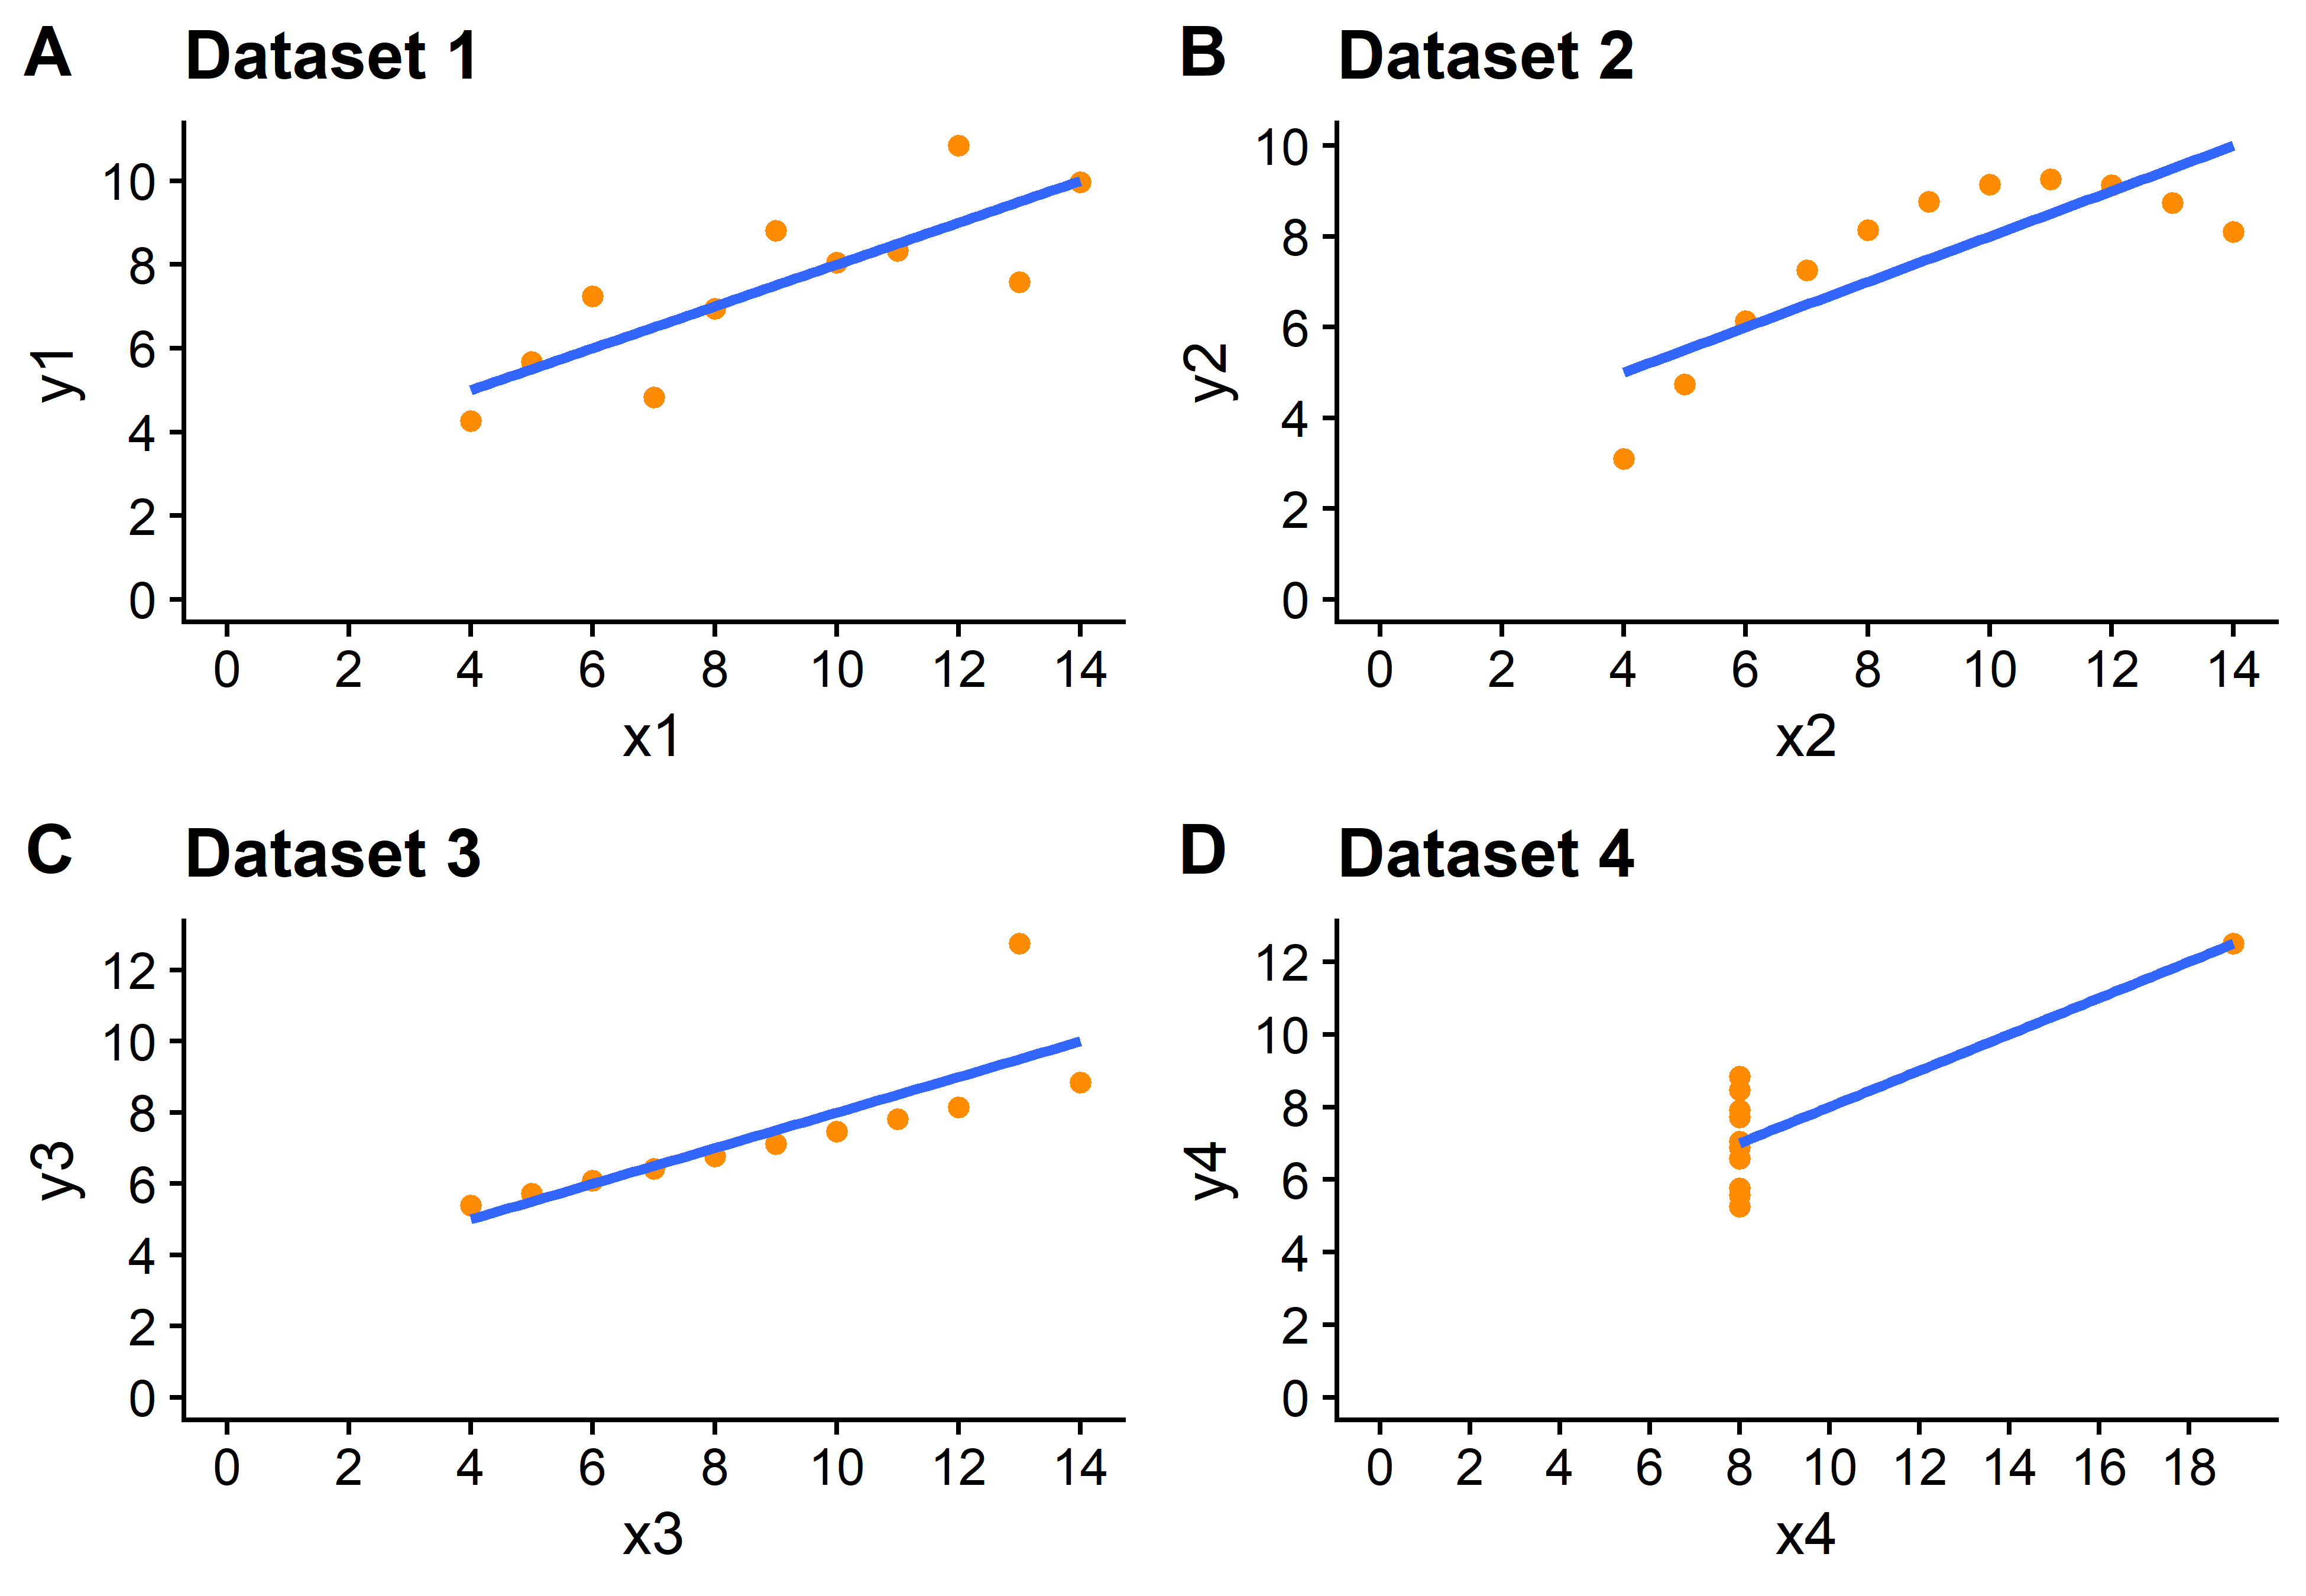
\includegraphics[width=1\linewidth]{images/anscombe2-1} 

}

\caption{O Quarteto de Anscombe}\label{fig:anscombe2}
\end{figure}
\bcenter

Fonte: do Autor.
\ecenter

\hypertarget{resultados}{%
\chapter{Resultados}\label{resultados}}

O pacote \pkg{stargazer} \autocite*{R-stargazer} é um dos melhores para a elaboração de tabelas de
coeficientes e estatísticas de modelos, conforme pode ser visto na tabela
\ref{tab:fits}:
\begin{table}[!htbp] \centering 
  \caption{Comparação entre diferentes quantis da regressão quantílica.} 
  \label{tab:fits} 
\begin{tabular}{@{\extracolsep{5pt}}lcc} 
\\[-1.8ex]\hline 
\hline \\[-1.8ex] 
 & \multicolumn{2}{c}{\textit{Dependent variable:}} \\ 
\cline{2-3} 
\\[-1.8ex] & \multicolumn{2}{c}{log(valor)} \\ 
\\[-1.8ex] & (1) & (2)\\ 
\hline \\[-1.8ex] 
 Constant & 13,56 (13,18, 13,94) & 13,60 (13,21, 13,99) \\ 
  & t = 58,85$^{***}$ & t = 57,70$^{***}$ \\ 
  area\_total & 0,001 (0,001, 0,002) & 0,002 (0,001, 0,002) \\ 
  & t = 5,11$^{***}$ & t = 5,23$^{***}$ \\ 
  quartos & 0,16 (0,11, 0,22) & 0,18 (0,12, 0,24) \\ 
  & t = 4,63$^{***}$ & t = 5,07$^{***}$ \\ 
  garagens & 0,21 (0,15, 0,26) & 0,23 (0,18, 0,28) \\ 
  & t = 6,25$^{***}$ & t = 7,28$^{***}$ \\ 
  suites & 0,06 (0,01, 0,12) &  \\ 
  & t = 1,81$^{***}$ &  \\ 
  log(dist\_b\_mar) & $-$0,14 ($-$0,19, $-$0,10) & $-$0,15 ($-$0,19, $-$0,10) \\ 
  & t = $-$5,17$^{***}$ & t = $-$5,31$^{***}$ \\ 
  I(padrao$\hat{\mkern6mu}$-1) & $-$0,56 ($-$0,74, $-$0,39) & $-$0,60 ($-$0,77, $-$0,42) \\ 
  & t = $-$5,36$^{***}$ & t = $-$5,63$^{***}$ \\ 
 \hline \\[-1.8ex] 
Observations & 48 & 48 \\ 
R$^{2}$ & 0,96 & 0,95 \\ 
Adjusted R$^{2}$ & 0,95 & 0,95 \\ 
Residual Std. Error & 0,14 (df = 41) & 0,14 (df = 42) \\ 
F Statistic & 148,92$^{***}$ (df = 6; 41) & 168,90$^{***}$ (df = 5; 42) \\ 
\hline 
\hline \\[-1.8ex] 
\textit{Note:}  & \multicolumn{2}{r}{$^{*}$p$<$0,3; $^{**}$p$<$0,2; $^{***}$p$<$0,1} \\ 
 & \multicolumn{2}{r}{Intervalos de Confiança de 90\% para os regressores.} \\ 
 & \multicolumn{2}{r}{Fonte: do Autor.} \\ 
\end{tabular} 
\end{table}
\hypertarget{conclusuxe3o}{%
\chapter{Conclusão}\label{conclusuxe3o}}

As conclusões devem responder às questões da pesquisa, em relação aos objetivos
e às hipóteses. Devem ser breves, podendo apresentar recomendações e sugestões
para trabalhos futuros.

\postextual

\begingroup

\printbibliography[title=REFERÊNCIAS]

\endgroup

\markboth{Referências}{REFERÊNCIAS}

\hypertarget{refs}{}
\begin{CSLReferences}{0}{0}
\end{CSLReferences}
\bapendices

\hypertarget{appendix-a}{%
\chapter{DESCRIÇÃO 1}\label{appendix-a}}

Textos elaborados pelo autor, a fim de completar a sua argumentação. Deve ser
precedido da palavra APÊNDICE, identificada por letras maiúsculas consecutivas,
travessão e pelo respectivo título. Utilizam-se letras maiúsculas dobradas quando
esgotadas as letras do alfabeto.

\textbf{No arquivo Rmd principal}
\begin{Shaded}
\begin{Highlighting}[]
\NormalTok{knitr}\SpecialCharTok{::}\NormalTok{opts\_chunk}\SpecialCharTok{$}\FunctionTok{set}\NormalTok{(}\AttributeTok{echo =} \ConstantTok{FALSE}\NormalTok{, }\AttributeTok{cache =} \ConstantTok{FALSE}\NormalTok{, }\AttributeTok{message=}\ConstantTok{FALSE}\NormalTok{, }
                      \AttributeTok{warning =} \ConstantTok{FALSE}\NormalTok{, }\AttributeTok{fig.ext=}\StringTok{\textquotesingle{}png\textquotesingle{}}\NormalTok{, }\AttributeTok{fig.align=}\StringTok{\textquotesingle{}center\textquotesingle{}}\NormalTok{, }
                      \AttributeTok{fig.path =} \StringTok{"images/"}\NormalTok{, }\AttributeTok{fig.pos =} \StringTok{"H"}\NormalTok{, }\AttributeTok{dev =} \StringTok{"png"}\NormalTok{, }
                      \AttributeTok{dpi =} \DecValTok{600}\NormalTok{, }\AttributeTok{out.width =} \StringTok{"70\%"}\NormalTok{)}
\NormalTok{type }\OtherTok{\textless{}{-}}\NormalTok{ knitr}\SpecialCharTok{::}\NormalTok{opts\_knit}\SpecialCharTok{$}\FunctionTok{get}\NormalTok{(}\StringTok{"rmarkdown.pandoc.to"}\NormalTok{)}
\CommentTok{\# This chunk ensures that the ufscdown package is}
\CommentTok{\# installed and loaded. This ufscdown package includes}
\CommentTok{\# the template files for the thesis.}
\ControlFlowTok{if}\NormalTok{(}\SpecialCharTok{!}\FunctionTok{require}\NormalTok{(remotes))}
  \FunctionTok{install.packages}\NormalTok{(}\StringTok{"remotes"}\NormalTok{, }\AttributeTok{repos =} \StringTok{"http://cran.rstudio.com"}\NormalTok{)}
\ControlFlowTok{if}\NormalTok{(}\SpecialCharTok{!}\FunctionTok{require}\NormalTok{(ufscdown))}
\NormalTok{  remotes}\SpecialCharTok{::}\FunctionTok{install\_github}\NormalTok{(}\StringTok{"lfpdroubi/ufscdown"}\NormalTok{)}
\FunctionTok{library}\NormalTok{(ufscdown)}
\end{Highlighting}
\end{Shaded}
\textbf{No Capítulo \ref{desenvolvimento}:}
\begin{Shaded}
\begin{Highlighting}[]
\FunctionTok{library}\NormalTok{(knitr)}
\ControlFlowTok{if}\NormalTok{(}\SpecialCharTok{!}\FunctionTok{require}\NormalTok{(kableExtra))}
  \FunctionTok{install.packages}\NormalTok{(}\StringTok{"kableExtra"}\NormalTok{, }\AttributeTok{repos =} \StringTok{"http://cran.rstudio.com"}\NormalTok{)}
\FunctionTok{library}\NormalTok{(kableExtra)}
\FunctionTok{kable}\NormalTok{(dados, }\AttributeTok{format =} \StringTok{"latex"}\NormalTok{, }\AttributeTok{booktabs =} \ConstantTok{TRUE}\NormalTok{,}
      \AttributeTok{caption =} \StringTok{"Médias concentrações urbanas 2010{-}2011."}\NormalTok{,}
      \AttributeTok{col.names =} \FunctionTok{c}\NormalTok{(}\StringTok{"Nome"}\NormalTok{, }\StringTok{"Total"}\NormalTok{, }\StringTok{"No Brasil"}\NormalTok{, }\StringTok{"Produto Interno Bruto {-} PIB"}\NormalTok{, }
                    \StringTok{"Número de Empresas"}\NormalTok{, }\StringTok{"Número de unidades locais"}\NormalTok{),}
      \AttributeTok{format.args =} \FunctionTok{list}\NormalTok{(}\AttributeTok{decimal.mark =} \StringTok{","}\NormalTok{, }\AttributeTok{big.mark =} \StringTok{" "}\NormalTok{)}
\NormalTok{    ) }\SpecialCharTok{\%\textgreater{}\%}
  \FunctionTok{kable\_styling}\NormalTok{(}\AttributeTok{latex\_options =} \StringTok{"striped"}\NormalTok{) }\SpecialCharTok{\%\textgreater{}\%} 
  \FunctionTok{add\_header\_above}\NormalTok{(}\FunctionTok{c}\NormalTok{(}\StringTok{"Média Concentração Urbana"}\NormalTok{, }\StringTok{"População"} \OtherTok{=} \DecValTok{2}\NormalTok{), }
                   \AttributeTok{bold =} \ConstantTok{TRUE}\NormalTok{) }\SpecialCharTok{\%\textgreater{}\%} 
  \FunctionTok{column\_spec}\NormalTok{(}\DecValTok{4}\SpecialCharTok{:}\DecValTok{6}\NormalTok{, }\AttributeTok{width =} \StringTok{"1.5cm"}\NormalTok{) }\SpecialCharTok{\%\textgreater{}\%} 
  \FunctionTok{row\_spec}\NormalTok{(}\DecValTok{0}\NormalTok{, }\AttributeTok{bold =} \ConstantTok{TRUE}\NormalTok{) }\SpecialCharTok{\%\textgreater{}\%} 
  \FunctionTok{footnote}\NormalTok{(}\AttributeTok{general =} \FunctionTok{c}\NormalTok{(}\StringTok{"PIB em bilhões de reais."}\NormalTok{, }\StringTok{"Fonte: IBGE (2016)"}\NormalTok{),}
           \AttributeTok{general\_title =} \StringTok{"Notas:"}\NormalTok{)}
\end{Highlighting}
\end{Shaded}
\hypertarget{appendix-b}{%
\chapter{FOR FUN}\label{appendix-b}}

\eapendices

\banexos

\hypertarget{descriuxe7uxe3o-1}{%
\chapter{DESCRIÇÃO 1}\label{descriuxe7uxe3o-1}}

São documentos não elaborados pelo autor que servem como fundamentação (mapas,
leis, estatutos). Deve ser precedido da palavra ANEXO, identificada por letras
maiúsculas consecutivas, travessão e pelo respectivo título. Utilizam-se letras
maiúsculas dobradas quando esgotadas as letras do alfabeto.

\textbf{No arquivo Rmd principal}
\begin{Shaded}
\begin{Highlighting}[]
\NormalTok{knitr}\SpecialCharTok{::}\NormalTok{opts\_chunk}\SpecialCharTok{$}\FunctionTok{set}\NormalTok{(}\AttributeTok{echo =} \ConstantTok{FALSE}\NormalTok{, }\AttributeTok{cache =} \ConstantTok{FALSE}\NormalTok{, }\AttributeTok{message=}\ConstantTok{FALSE}\NormalTok{, }
                      \AttributeTok{warning =} \ConstantTok{FALSE}\NormalTok{, }\AttributeTok{fig.ext=}\StringTok{\textquotesingle{}png\textquotesingle{}}\NormalTok{, }\AttributeTok{fig.align=}\StringTok{\textquotesingle{}center\textquotesingle{}}\NormalTok{, }
                      \AttributeTok{fig.path =} \StringTok{"images/"}\NormalTok{, }\AttributeTok{fig.pos =} \StringTok{"H"}\NormalTok{, }\AttributeTok{dev =} \StringTok{"png"}\NormalTok{, }
                      \AttributeTok{dpi =} \DecValTok{600}\NormalTok{, }\AttributeTok{out.width =} \StringTok{"70\%"}\NormalTok{)}
\NormalTok{type }\OtherTok{\textless{}{-}}\NormalTok{ knitr}\SpecialCharTok{::}\NormalTok{opts\_knit}\SpecialCharTok{$}\FunctionTok{get}\NormalTok{(}\StringTok{"rmarkdown.pandoc.to"}\NormalTok{)}
\CommentTok{\# This chunk ensures that the ufscdown package is}
\CommentTok{\# installed and loaded. This ufscdown package includes}
\CommentTok{\# the template files for the thesis.}
\ControlFlowTok{if}\NormalTok{(}\SpecialCharTok{!}\FunctionTok{require}\NormalTok{(remotes))}
  \FunctionTok{install.packages}\NormalTok{(}\StringTok{"remotes"}\NormalTok{, }\AttributeTok{repos =} \StringTok{"http://cran.rstudio.com"}\NormalTok{)}
\ControlFlowTok{if}\NormalTok{(}\SpecialCharTok{!}\FunctionTok{require}\NormalTok{(ufscdown))}
\NormalTok{  remotes}\SpecialCharTok{::}\FunctionTok{install\_github}\NormalTok{(}\StringTok{"lfpdroubi/ufscdown"}\NormalTok{)}
\FunctionTok{library}\NormalTok{(ufscdown)}
\end{Highlighting}
\end{Shaded}
\textbf{No Capítulo \ref{ref-labels}:}
\begin{Shaded}
\begin{Highlighting}[]
\FunctionTok{library}\NormalTok{(knitr)}
\ControlFlowTok{if}\NormalTok{(}\SpecialCharTok{!}\FunctionTok{require}\NormalTok{(kableExtra))}
  \FunctionTok{install.packages}\NormalTok{(}\StringTok{"kableExtra"}\NormalTok{, }\AttributeTok{repos =} \StringTok{"http://cran.rstudio.com"}\NormalTok{)}
\FunctionTok{library}\NormalTok{(kableExtra)}
\FunctionTok{kable}\NormalTok{(dados, }\AttributeTok{format =} \StringTok{"latex"}\NormalTok{, }\AttributeTok{booktabs =} \ConstantTok{TRUE}\NormalTok{,}
      \AttributeTok{caption =} \StringTok{"Médias concentrações urbanas 2010{-}2011."}\NormalTok{,}
      \AttributeTok{col.names =} \FunctionTok{c}\NormalTok{(}\StringTok{"Nome"}\NormalTok{, }\StringTok{"Total"}\NormalTok{, }\StringTok{"No Brasil"}\NormalTok{, }\StringTok{"Produto Interno Bruto {-} PIB"}\NormalTok{, }
                    \StringTok{"Número de Empresas"}\NormalTok{, }\StringTok{"Número de unidades locais"}\NormalTok{),}
      \AttributeTok{format.args =} \FunctionTok{list}\NormalTok{(}\AttributeTok{decimal.mark =} \StringTok{","}\NormalTok{, }\AttributeTok{big.mark =} \StringTok{" "}\NormalTok{)}
\NormalTok{    ) }\SpecialCharTok{\%\textgreater{}\%}
  \FunctionTok{kable\_styling}\NormalTok{(}\AttributeTok{latex\_options =} \StringTok{"striped"}\NormalTok{) }\SpecialCharTok{\%\textgreater{}\%} 
  \FunctionTok{add\_header\_above}\NormalTok{(}\FunctionTok{c}\NormalTok{(}\StringTok{"Média Concentração Urbana"}\NormalTok{, }\StringTok{"População"} \OtherTok{=} \DecValTok{2}\NormalTok{), }
                   \AttributeTok{bold =} \ConstantTok{TRUE}\NormalTok{) }\SpecialCharTok{\%\textgreater{}\%} 
  \FunctionTok{column\_spec}\NormalTok{(}\DecValTok{4}\SpecialCharTok{:}\DecValTok{6}\NormalTok{, }\AttributeTok{width =} \StringTok{"1.5cm"}\NormalTok{) }\SpecialCharTok{\%\textgreater{}\%} 
  \FunctionTok{row\_spec}\NormalTok{(}\DecValTok{0}\NormalTok{, }\AttributeTok{bold =} \ConstantTok{TRUE}\NormalTok{) }\SpecialCharTok{\%\textgreater{}\%} 
  \FunctionTok{footnote}\NormalTok{(}\AttributeTok{general =} \FunctionTok{c}\NormalTok{(}\StringTok{"PIB em bilhões de reais."}\NormalTok{, }\StringTok{"Fonte: IBGE (2016)"}\NormalTok{),}
           \AttributeTok{general\_title =} \StringTok{"Notas:"}\NormalTok{)}
\end{Highlighting}
\end{Shaded}
\hypertarget{for-fun}{%
\chapter{for Fun}\label{for-fun}}

\eanexos

% ----------------------------------------------------------
% Glossário
% ----------------------------------------------------------
%
% Consulte o manual da classe abntex2 para orientações sobre o glossário.
%
%\glossary

%---------------------------------------------------------------------
% INDICE REMISSIVO
%---------------------------------------------------------------------
%\phantompart
%\printindex
%---------------------------------------------------------------------

\end{document}
